% main.tex -- демонстрационный шаблон ВКР ИТМО
% "Разработка инструмента планирования миграции кодовой базы проекта на алгоритмы постквантовой криптографии"

\documentclass{itmo-vkr}

%\usepackage{listings}
\usepackage{xcolor}
\usepackage{float}
\usepackage{graphicx}
\graphicspath{{figures/}}  % изображения в папке figures/
\usepackage{tikz}
\usetikzlibrary{shapes.geometric,arrows.meta,positioning}

% BibLaTeX + Biber + ГОСТ-стиль уже подключены в классе, здесь указываем .bib
\addbibresource{references.bib}

% Команда для имён функций/классов/тестов: курсив по ГОСТ
% (\setmonofont = Times New Roman, поэтому \texttt = основной шрифт;
%  Menlo используется только внутри itmolisting, а \textit даёт нужное выделение)
\newcommand{\code}[1]{\textit{#1}}

% Определение языка JSON для листингов
\lstdefinelanguage{JSON}{
  basicstyle=\itmoListingFont\small,
  morestring=[b]",
  morecomment=[l]{//},
  morecomment=[s]{/*}{*/},
  literate=
    *{0}{{{\color{blue}0}}}{1}
     {1}{{{\color{blue}1}}}{1}
     {2}{{{\color{blue}2}}}{1}
     {3}{{{\color{blue}3}}}{1}
     {4}{{{\color{blue}4}}}{1}
     {5}{{{\color{blue}5}}}{1}
     {6}{{{\color{blue}6}}}{1}
     {7}{{{\color{blue}7}}}{1}
     {8}{{{\color{blue}8}}}{1}
     {9}{{{\color{blue}9}}}{1}
     {:}{{{\color{gray}{:}}}}{1}
     {,}{{{\color{gray}{,}}}}{1}
     {\{}{{{\color{black}{\{}}}}{1}
     {\}}{{{\color{black}{\}}}}}{1}
     {[}{{{\color{black}{[}}}}{1}
     {]}{{{\color{black}{]}}}}{1},
}

\title{Разработка инструмента планирования миграции кодовой базы проекта на алгоритмы постквантовой криптографии}
\author{Пронина А. И.}
\date{2026}

\begin{document}
	
	% === СОДЕРЖАНИЕ ===
	\tableofcontents
	\newpage
	
	% === СПИСОК СОКРАЩЕНИЙ ===
	\unnumberedchapter{СПИСОК СОКРАЩЕНИЙ И УСЛОВНЫХ ОБОЗНАЧЕНИЙ}
	
	\begin{abbreviations}
		\abbritem{AES}{Advanced Encryption Standard -- расширенный стандарт симметричного шифрования}
		\abbritem{API}{Application Programming Interface -- интерфейс прикладного программирования}
		\abbritem{AST}{Abstract Syntax Tree -- абстрактное синтаксическое дерево}
		\abbritem{BFS}{Breadth-First Search -- обход графа в ширину}
		\abbritem{CBOM}{Cryptography Bill of Materials -- криптографическая ведомость материалов}
		\abbritem{CLI}{Command Line Interface -- интерфейс командной строки}
		\abbritem{DER}{Distinguished Encoding Rules -- правила однозначного кодирования ASN.1}
		\abbritem{DH/DHE}{Diffie-Hellman (Ephemeral) -- (эфемерный) обмен ключами Диффи-Хеллмана}
		\abbritem{DSA}{Digital Signature Algorithm -- алгоритм цифровой подписи}
		\abbritem{ECC}{Elliptic Curve Cryptography -- криптография на эллиптических кривых}
		\abbritem{ECDH}{Elliptic Curve Diffie-Hellman -- обмен ключами на эллиптических кривых}
		\abbritem{ECDSA}{Elliptic Curve Digital Signature Algorithm -- алгоритм цифровой подписи на ЭК}
		\abbritem{FIPS}{Federal Information Processing Standard -- федеральный стандарт обработки информации (США)}
		\abbritem{FN}{False Negative -- ложноотрицательный результат}
		\abbritem{FP}{False Positive -- ложноположительный результат}
		\abbritem{HNDL}{Harvest Now, Decrypt Later -- атака «собери сейчас, расшифруй потом»}
		\abbritem{JSON}{JavaScript Object Notation -- текстовый формат обмена данными}
		\abbritem{KEM}{Key Encapsulation Mechanism -- механизм инкапсуляции ключей}
		\abbritem{MD5}{Message Digest Algorithm 5 -- криптографическая хеш-функция}
		\abbritem{ML-DSA}{Module Lattice-Based Digital Signature Algorithm -- алгоритм ЦП на модульных решётках (FIPS~204)}
		\abbritem{ML-KEM}{Module Lattice-Based Key Encapsulation Mechanism -- механизм инкапсуляции ключей на модульных решётках (FIPS~203)}
		\abbritem{NIST}{National Institute of Standards and Technology -- Национальный институт стандартов и технологий США}
		\abbritem{PEM}{Privacy-Enhanced Mail -- формат кодирования криптографических объектов (Base64)}
		\abbritem{PKI}{Public Key Infrastructure -- инфраструктура открытых ключей}
		\abbritem{PQC}{Post-Quantum Cryptography -- постквантовая криптография}
		\abbritem{RSA}{Rivest--Shamir--Adleman -- алгоритм асимметричного шифрования и цифровой подписи}
		\abbritem{SBOM}{Software Bill of Materials -- ведомость программных компонентов}
		\abbritem{SHA}{Secure Hash Algorithm -- алгоритм безопасного хеширования}
		\abbritem{SLH-DSA}{Stateless Hash-Based Digital Signature Algorithm -- алгоритм ЦП на хеш-функциях без состояния (FIPS~205)}
		\abbritem{TLS}{Transport Layer Security -- протокол защиты транспортного уровня}
		\abbritem{TP}{True Positive -- истинно положительный результат}
		\abbritem{ГОСТ}{Государственный стандарт}
		\abbritem{ТК~26}{Технический комитет по стандартизации «Криптографическая защита информации»}
	\end{abbreviations}
	
	% === ТЕРМИНЫ И ОПРЕДЕЛЕНИЯ ===
	\unnumberedchapter{ТЕРМИНЫ И ОПРЕДЕЛЕНИЯ}
	
	\begin{termlist}
		\termitem{Квантово-уязвимый алгоритм}
		{
			криптографический алгоритм, безопасность которого может быть нарушена за полиномиальное время с использованием квантового компьютера достаточной мощности.
		}
		
		\termitem{Постквантовая криптография}{
			раздел криптографии, посвящённый разработке криптографических алгоритмов, устойчивых к атакам как классических, так и квантовых компьютеров.
		}
		
		\termitem{Криптографический манифест (CBOM)}{
			расширение формата CycloneDX Software Bill of Materials, описывающее криптографические активы программной системы: алгоритмы, ключи, сертификаты и протоколы.
		}
		
		\termitem{Статический анализ}{
			метод проверки программного кода без его выполнения, позволяющий выявлять дефекты, уязвимости и использование устаревших API.
		}
		
		\termitem{Инкапсуляция ключей (KEM)}{
			криптографический примитив, позволяющий безопасно передавать симметричный ключ с использованием асимметричной криптографии.
		}
		
		\termitem{Криптографическая гибкость (Crypto-Agility)}{
			свойство программной системы, позволяющее заменять криптографические алгоритмы без существенной переработки архитектуры.
		}
	\end{termlist}
	
	\newpage
	
	% === ВВЕДЕНИЕ (как структурный элемент без номера) ===
	\unnumberedchapter{ВВЕДЕНИЕ}
	
	В настоящее время стремительное развитие квантовых вычислений формирует совершенно новый класс угроз для современной криптографической инфраструктуры. В частности, алгоритм Шора, запущенный на квантовом компьютере, способен за полиномиальное время (со сложностью $O(n^k)$, что означает быструю работу за минуты или часы вместо десятков лет) взломать любую стандартную систему с открытым ключом, что разрушает фундамент современной асимметричной криптографии: RSA, ECDSA и протокол Диффи-Хеллмана~\cite{1994Shor}.
	
	Согласно ежегодному докладу Global Risk Institute за 2025-2026 год, вероятность появления криптографически значимого квантового компьютера в течение ближайших десяти лет составляет от 28\% до 49\%, что является максимальным показателем за семилетнюю историю публикаций~\cite{mosca2025timeline}. По оценкам ведущих исследовательских центров, создание квантового компьютера с числом логических кубитов, достаточным для взлома RSA-2048 в реальные сроки (от 1 дня до недели)\cite{gidney2025million}, прогнозируется в период 2030-2040 годов~\cite{IBMRoadmap2026}\cite{TQI_GoogleRoadmap2026}. 
	
	В ответ на эту угрозу Национальный институт стандартов и технологий США (NIST) в августе 2024 года опубликовал первые три финализированных стандарта постквантовой криптографии: FIPS 203, FIPS 204 и FIPS 205 ~\cite{nist-fips203}\cite{nist-fips204}\cite{nist-fips205}. На российском рынке ТК 26 ведет активную работу по разработке отечественных постквантовых алгоритмов: электронной подписи "Шиповник" и "Гиперикум", а также механизма инкапсуляции ключей "Кодиеум"~\cite{kryptonite-codiaeum}\cite{qapp-hypericum}.
	
	Вопрос инвентаризации криптографических активов в профильной аналитике уже рассматривается как одно из ключевых узких мест постквантовой подготовки. Совместный отчёт IBM Institute for Business Value и Cloud Security Alliance \textit{Secure the post-quantum future}~\cite{IBM_Secure_PQ_2025} фиксирует, что криптографическая инвентаризация по-прежнему остаётся эпизодической практикой: по данным опроса, лишь около 30\,\% организаций завершили инвентаризацию приложений, данных и сервисов с целью понять, как именно используется в них криптография, а только 24\,\% применяют полученные результаты для трансформации своих бизнес-процессов. Авторы подчёркивают, что криптографический инвентарь должен давать «полную карту криптографических реализаций и зависимостей» и является «критически важным стартовым шагом» для разработки дорожной карты перехода к квантово-устойчивым решениям, однако на практике большинство организаций не доходят до этого шага.
	
	Непосредственный переход к алгоритмам постквантовой криптографии представляет собой масштабную инженерную задачу. Современные программные системы содержат тысячи вызовов криптографических функций, распределенных по десяткам файлов с исходным кодом. Ручная проверка подобной кодовой базы представляет собой весьма трудоемкий, подверженный ошибкам процесс, который очень плохо масштабируется на крупные проекты. В связи с этим возникает потребность в специализированном инструменте, способном автоматически обнаруживать уязвимые вызовы, оценивать их критичность в контексте конкретного программного решения, а затем формировать приоритизированный план миграции в соответствии с действующими отечественными и мировыми стандартами.
	
	\textbf{Целью данной работы} является автоматизация процесса оценки и планирования миграции к постквантовым криптографическим алгоритмам посредством выявления квантово-уязвимых решений и формирования плана их модернизации на основе стандартов NIST с учетом развития отечественной нормативной базы ТК 26.
	
	Для достижения поставленной цели должны быть решены следующие \textbf{задачи}:
	
	\begin{enumerate}
		\item Провести анализ квантовых угроз для современной криптографии, изучить профильные стандарты и выявить ограничения существующих аналогов разрабатываемого программного обеспечения.
		\item Спроектировать модульную архитектуру инструмента и базу данных сигнатур, содержащую параметры уязвимых API-функций, форматы данных и структуру отчетов.
		\item Реализовать программные модули инвентаризации файлов проекта и статического анализа кода для извлечения вызовов криптографических функций и анализа сертификатов.
		\item Реализовать модули оценки рисков и планирования миграции на рекомендуемые постквантовые аналоги.
		\item Провести функциональное тестированние на контрольной кодовой базе, проанализировать точность обнаружения.
		
	\end{enumerate}
	
	В ходе выполнения данной работы был предложен и реализован программный инструмент, предназначенный для автоматической инвентаризации криптографических активов в программных системах и оценки сопряжённых с ними квантовых рисков. Практическая значимость работы определяется тем, что инструмент позволяет без ручного вмешательства выявлять квантово-уязвимые криптографические решения в исходном коде и формировать приоритизированный план их миграции в соответствии с рекомендациями NIST и ТК 26. Личный вклад автора состоит в проектировании архитектуры инструмента, разработке базы данных криптографических сигнатур, а также в программной реализации модулей статического анализа, оценки рисков и планирования миграции.
	
	
	
	
	\section{Анализ квантовых угроз и нормативной базы}
	
	\subsection{Основы современной криптографии}
	
	
	Криптография (от греч. κρυπτός -- скрытый и γράφω -- пишу) -- наука о методах обеспечения конфиденциальности, целостности и аутентичности информации посредством математических преобразований. В современном понимании криптография решает четыре фундаментальные задачи: конфиденциальность (невозможность прочитать сообщение без ключа), целостность (обнаружение несанкционированных изменений), аутентификация (подтверждение источника данных) и неотказуемость (невозможность отрицать авторство).
	
	Принцип Керкгоффса, сформулированный в 1883 году, утверждает: стойкость криптосистемы не должна зависеть от секретности алгоритма -- только от секретности ключа. Этот принцип лежит в основе всех современных стандартов, включая те, которые анализируются в данной работе.
	
	\textit{Симметричная криптография}
	
	Симметричные алгоритмы шифрования используют один и тот же секретный ключ для шифрования и дешифрования данных. Основные достоинства -- высокая скорость и вычислительная эффективность, что делает симметричные шифры предпочтительными для шифрования больших объёмов данных.
	
	Эталонным стандартом симметричного шифрования является AES (Advanced Encryption Standard), принятый NIST в 2001 году (FIPS 197). AES работает с блоками данных длиной 128 бит и поддерживает ключи трёх размеров: 128, 192 и 256 бит. Алгоритм основан на сети подстановок-перестановок (SPN) и применяет 10, 12 или 14 раундов обработки соответственно. AES-256 обеспечивает 256-битный уровень классической стойкости и в настоящее время рекомендован NIST как долгосрочный стандарт.
	
	Главная проблема симметричных систем -- задача распределения ключей: обеим сторонам необходимо заранее договориться о секретном ключе по защищённому каналу. Именно для решения этой проблемы была разработана асимметричная криптография.
	
	\textit{Асимметричная криптография}
	
	Асимметричные, или системы с открытым ключом, используют пару математически связанных ключей: открытый (публичный) ключ, доступный всем, и закрытый (приватный) ключ, известный только владельцу. Сообщение, зашифрованное открытым ключом, может быть расшифровано только соответствующим закрытым ключом, и наоборот.
	
	Концепция асимметричной криптографии была введена в 1976 году Диффи и Хеллманом в работе «New Directions in Cryptography», а в 1977 году Ривест, Шамир и Адлеман предложили первую практическую реализацию -- алгоритм RSA. RSA основан на вычислительной сложности задачи факторизации больших целых чисел: произведение $N = p \cdot q$ двух больших простых чисел $p$ и $q$ легко вычислить, но крайне сложно разложить обратно.
	
	Другой фундаментальной асимметричной операцией является протокол Диффи-Хеллмана (DH) для обмена ключами, стойкость которого основана на сложности задачи дискретного логарифмирования в конечных полях. Более компактный вариант -- криптография на эллиптических кривых (ECC): ECDH (обмен ключами) и ECDSA (цифровая подпись) -- опирается на задачу дискретного логарифмирования на эллиптических кривых (ECDLP) и обеспечивает эквивалентный RSA уровень стойкости при значительно меньшем размере ключа.
	
	Асимметричные алгоритмы существенно медленнее симметричных. Поэтому на практике применяется гибридная схема: асимметричная криптография используется лишь для защищённой передачи симметричного ключа сессии, а сами данные шифруются быстрым симметричным алгоритмом (AES). Именно так работают протоколы TLS, SSH и большинство современных систем защиты коммуникаций.
	
	\textit{Гибридное шифрование: совместная работа симметричных и асимметричных систем}
	
	На практике симметричная и асимметричная криптография не конкурируют, а дополняют друг друга в рамках гибридной схемы шифрования, которая устраняет недостатки обоих подходов одновременно.
	
	Проблема симметричной криптографии -- распределение ключей: прежде чем зашифровать данные, обе стороны должны согласовать секретный ключ по защищённому каналу, которого изначально не существует. Асимметричная криптография решает эту проблему, но платит за это производительностью: RSA или ECDH на несколько порядков медленнее AES, и шифровать большие объёмы данных асимметричным алгоритмом неприемлемо.
	
	Гибридная схема работает следующим образом:
	
	\begin{enumerate}
		\item Получатель (Боб) заранее публикует свой открытый ключ (RSA или ECDH).
		\item Отправитель (Алиса) генерирует одноразовый симметричный сеансовый ключ (например, 256-битный AES).
		\item Алиса шифрует сеансовый ключ открытым ключом Боба (асимметричная операция -- небольшой объём данных, выполняется быстро).
		\item Алиса шифрует сами данные сеансовым ключом AES (симметричная операция -- высокая скорость при любом объёме).
		\item Боб расшифровывает сеансовый ключ своим закрытым ключом и затем расшифровывает данные.
		
	\end{enumerate}
	
	Таким образом, асимметричная криптография применяется только для передачи одного небольшого объекта -- ключа, -- а весь реальный трафик защищается быстрым симметричным алгоритмом.
	
	Именно так устроен протокол TLS (Transport Layer Security), защищающий HTTPS, SMTP и большинство других защищённых протоколов. На этапе TLS-рукопожатия (handshake) клиент и сервер используют асимметричную криптографию (RSA или ECDHE) для выработки общего premaster secret, из которого обе стороны независимо выводят одинаковый сеансовый ключ (session key). После завершения рукопожатия весь дальнейший трафик шифруется этим симметричным ключом.
	
	
	\textit{Хеш-функции и цифровая подпись}
	
	Криптографическая хеш-функция -- это детерминированная функция $H : \{0, 1\}* \rightarrow \{0, 1\}^n$, отображающая входные данные произвольной длины в строку фиксированной длины (хеш-сумма). Криптографически стойкая хеш-функция должна обладать тремя свойствами:
	
	
	\begin{itemize}
		\item Однонаправленность: зная $H(M)$, практически невозможно восстановить $M$.
		\item Устойчивость к коллизиям: практически невозможно найти два различных сообщения $M \neq M'$ такие, что $H(M) = H(M')$.
		\item Устойчивость ко второму прообразу: зная $M$ и $H(M)$, практически невозможно найти $M' \neq M$ с $H(M) = H(M')$.
	\end{itemize}
	
	Широко применяемые алгоритмы: SHA-256 (семейство SHA-2, 256-битная хем-сумма, рекомендуется NIST), SHA-1 (160 бит, устаревший, небезопасен для цифровых подписей с 2013 года по NIST SP 800-131A Rev.2), MD5 (128 бит, признан небезопасным). NIST запрещает использование MD5 и SHA-1 в новых протоколах.
	
	Цифровая подпись сочетает асимметричную криптографию с хеш-функцией: отправитель вычисляет хеш-сумму сообщения и шифрует его своим закрытым ключом; получатель проверяет подпись с помощью открытого ключа. Это обеспечивает одновременно аутентификацию источника и контроль целостности. Стандарты: ECDSA (основан на ECC), DSA (изъят из стандарта NIST FIPS 186-5 в 2023 году), RSA-PSS (на основе RSA).
	
	\textit{Инфраструктура открытых ключей (PKI)}
	
	На практике распределение открытых ключей реализуется через инфраструктуру открытых ключей (PKI) -- иерархическую систему центров сертификации (CA), которые выпускают цифровые сертификаты X.509. Сертификат связывает открытый ключ с его идентификационными данными и подписывается закрытым ключом CA, формируя цепочку доверия. Именно PKI обеспечивает безопасность HTTPS, TLS, S/MIME, SSH и других прикладных протоколов. Нарушение стойкости асимметричных алгоритмов, лежащих в основе PKI, потребует комплексной замены всей цепочки сертификатов -- этому аспекту уделяется особое внимание в части планирования миграции (глава 3 настоящей работы).
	
	
	\subsection{Квантовые вычисления как новый вектор угроз для современной криптографии}
	
	Современная криптографическая инфраструктура строится на предположении о вычислительной сложности определённых математических задач. 
	Асимметричные алгоритмы  --  RSA, протокол Диффи–Хеллмана (DH), алгоритмы на эллиптических кривых (ECDSA, ECDH, ГОСТ Р 34.10-2012)  --  обязаны своей безопасностью тому, что задачи целочисленной факторизации и дискретного логарифмирования вычислительно неразрешимы на обычном компьютере за разумное время. Лучший классический алгоритм -- метод решета числового поля -- работает за субэкспоненциальное время порядка $e^{O\left((\log N)^{1/3} (\log \log N)^{2/3}\right)}$, что делает прямые атаки практически невозможными в обозримом будущем при использовании стандартных вычислителей.
	
	Квантовые компьютеры принципиально нарушают этот баланс. В отличие от классических машин, они оперируют кубитами -- квантовыми битами, способными находиться в суперпозиции состояний. Квантовый параллелизм и явление запутанности позволяют реализовать алгоритмы, которые решают задачи факторизации и дискретного логарифмирования за полиномиальное время. На практике это означает, что весь класс задач, лежащих в основе современной асимметричной криптографии, становится критически уязвимым для достаточно мощного квантого компьютера.
	
	
	
	Практическая реализация данной угрозы долгое время не выходила за рамки научных расчетов: для взлома RSA-2048 требовалось несколько десятков миллионов физических кубитов, что еще не так давно казалось недостижимым. Однако в последние годы ситуация значительно изменилась. В декабре 2024 года компания Google представила процессор Willow со 105 свехпроводящими кубитами, впервые продемонстрировав возможность экспоненциального подавления ошибок при увеличении числа задействованных кубитов. Данный результат подтверждает принципиальную возможность создания отказоустойчивых систем, способных сохранять стабильность при масштабировании. В мае 2025 года исследователь Google Q
	uantum AI Крейг Гидни опубликовал работу, в которой показал, что факторизация ключа RSA-2048 потенциально достижима менее чем за одну неделю на квантовом компьютере с числом физических кубитов менее одного миллиона -- это в 20 раз меньше его же оценок времен 2019 года~\cite{gidney2025million}. Принципиально важно, что группа из Сиднея в 2026 году опубликовала ещё более оптимистичные оценки, утверждая о возможности взлома RSA-2048 менее чем при 100 000 физических кубитов~\cite{iceberg2026pinnacle}. Такого прорыва удалось достичь за счет отказа от поверхностной архитектуры коррекции ошибок в пользу квантовых LDPC-алгоритмов. Эта технология позволяет связывать кубиты в гибкую и эффективную сеть, что сокращает аппаратные затраты в десятки раз. 
	
	Согласно седьмому ежегодному докладу Global Risk Institute за 2025-2026 год~\cite{mosca2025timeline}, экспертное сообщество достигло исторического максимума в своих опасениях относительно квантовой угрозы: 26 ведущих мировых специалистов сошлись во мнении, что вероятность создания полноценного криптографически значимого квантового компьютера в ближайшее десятилетие составляет от 28\% до 49\%. В долгосрочной перспективе прогнозы становятся еще более определенными: на горизонте пятнадцати лет 69\% участников опроса оценивают вероятность появления такой машины как 50\% и выше; через 20 лет этот показатель достигает 92\%. Параллельно с этим, аналитическая модель Project Eleven устанавливает конкретные сроки для наступления «Q-Day» (момента краха современной криптографии). Согласно их расчетам, наиболее вероятный сценарий реализации этой угрозы приходится на 2033 год, однако при неблагоприятном развитии событий это может произойти уже в 2030 году.
	
	Угроза носит асимметричный характер: она нарастает не внезапно, а постепенно, и её наиболее опасный аспект разворачивается уже в данный момент -- задолго до появления первого криптографически значимого квантового компьютера.
	
	Теоретические основы квантовых вычислений, включая принципы суперпозиции, запутанности и квантового параллелизма, подробно рассматриваются в работе П.Г. Ключарева «Основы квантовых вычислений и квантовой криптографии»~\cite{klucharyov-osnovy-kvantovyh}. Автор акцентирует внимание на принципиальном отличии квантовых алгоритмов от классических: если классический компьютер обрабатывает состояния последовательно, квантовый процессор в силу суперпозиции способен одновременно находиться во всех $2^n$ состояниях при $n$ кубитах, что и обеспечивает экспоненциальное ускорение для определённых классов задач. Это теоретическое преимущество составляет физическую основу угроз, рассматриваемых в настоящей работе.
	
	\subsection{Алгоритм Шора: теоретическая угроза асимметричной криптографии}
	
	Алгоритм Шора был разработан американским математиком Питером Шором в 1994 году и в настоящее время считается наиболее опасным криптоаналитическим квантовым алгоритмом~\cite{1994Shor}. Его значимость состоит в том, что его автор впервые предложил способ решения задачи целочисленной факторизации за полиномиальное время $O(\log^3 N)$ при использовании $O(\log N)$ кубитов, а не за субэкспоненциальное, характерное для лучших классических методов~\cite{kvantovye-algoritmy-shor-grover}.
	
	Алгоритм состоит из двух частей -- классической и квантовой. Классическая часть сводит задачу факторизации числа 
	$N$ к задаче нахождения периода функции $f_a(x) = a^x \pmod{N}$
	где 
	$a$ -- случайное целое число, взаимно простое с $N$. Нахождение периода 
	$r$ этой функции позволяет вычислить $\gcd(a^{r/2} -- 1, N)$ и $\gcd(a^{r/2} + 1, N)$, которые с высокой вероятностью окажутся нетривиальными делителями 
	$N$. Именно задача нахождения периода, неэффективная на классических машинах, решается квантовой частью -- с помощью квантового преобразования Фурье (QFT). QFT реализует дискретное преобразование Фурье над амплитудами квантового состояния за $O((\log N)^2)$ операций, тогда как классическое быстрое преобразование Фурье (FFT) требует $O(N \log N)$. Это и обеспечивает экспоненциальное ускорение.
	
	Применительно к криптографии алгоритм Шора разрушает безопасность всех широко используемых асимметричных систем:
	
	\begin{itemize}
		\item \textbf{RSA} -- стойкость основана на сложности факторизации большого числа $N = p \cdot q$. Алгоритм Шора напрямую решает эту задачу.
		\item \textbf{ECDSA, ECDH} -- стойкость основана на сложности задачи дискретного логарифмирования в группе точек эллиптической кривой. Алгоритм Шора, будучи настроен на задачу дискретного логарифмирования, решает и её за полиномиальное время.
		\item \textbf{ГОСТ Р 34.10-2012} -- российский стандарт электронной подписи, также построенный на задаче дискретного логарифмирования в группе точек эллиптических кривых, оказывается уязвимым по той же причине.~\cite{kvantovyj-kompyuter-kriptostoykost}
		\item \textbf{Схема Диффи–Хеллмана (DH/ECDH)} -- протоколы обмена ключами, основанные на классической или эллиптической версии дискретного логарифмирования, также подпадают под действие алгоритма Шора.
	\end{itemize}
	
	Работоспособность алгоритма была экспериментально подтверждена в 2001 году при факторизации числа 15 на 7-кубитном квантовом компьютере. Достигнутые к 2020 году рекорды квантовой факторизации не превышали 41-битных чисел, что по-прежнему бесконечно далеко от RSA-2048. Однако принципиальным является не нынешнее состояние, а вектор развития. Снижение оценочного числа физических кубитов для взлома RSA-2048 от 20 миллионов в 2019 году до менее чем 1 миллиона в 2025 году демонстрирует, что ресурсные барьеры стремительно уменьшаются.
	
	Особую уязвимость проявляют системы на эллиптических кривых. По результатам ресурсного анализа Roetteler et al.~\cite{roetteler2017ecc}, для решения задачи дискретного логарифмирования на 256-битной кривой~(P-256) методом Шора достаточно около 2~330 логических кубитов. Для сравнения: классическая схема квантовой факторизации Бьюрегарда~\cite{beauregard2003circuit} требует $2n{+}3 = 4\,099$ логических кубитов при $n = 2048$ для RSA-2048, а более поздняя оптимизация~\cite{chevignard2024reducing} снижает эту оценку до 1~730 за счёт пространственно-временного компромисса~-- значительного увеличения числа квантовых вентилей при сокращении кубитов. Таким образом, ECC-системы требуют заметно меньших квантовых ресурсов для взлома, чем RSA, и могут оказаться уязвимыми раньше при равном уровне развития квантовых компьютеров.
	
	Критично понимать, что алгоритм Шора не затрагивает симметричные алгоритмы (AES, «Кузнечик») и хэш-функции (SHA, «Стрибог»), поскольку их безопасность не основана на задачах факторизации или дискретного логарифмирования. Однако, поскольку в современных протоколах симметричное шифрование неизменно применяется в связке с асимметричным (например, в TLS асимметрика используется для безопасного распределения симметричного сеансового ключа), компрометация асимметричного слоя фактически разрушает всю цепочку защиты.
	
	
	\subsection{Алгоритм Гровера: влияние на симметричную криптографию}
	
	Алгоритм Гровера, предложенный Ловом Гровером в 1996 году, представляет собой квантовый алгоритм поиска в неструктурированных базах данных. В контексте криптоанализа он применим к задаче перебора ключей симметричных шифров: вместо того чтобы перебирать все $2^n$ возможных ключей, квантовый вычислитель с помощью алгоритма Гровера способен найти ключ за $O(2^{n/2})$ операций. Иными словами, алгоритм обеспечивает квадратичное ускорение перебора, что эквивалентно уменьшению эффективной длины ключа вдвое. 
	
	Практические следствия для современных симметричных алгоритмов выглядят следующим образом:
	
	\begin{itemize}
		\item \textbf{AES-128} -- эффективная безопасность снижается с 128 бит до приблизительно 64 бит, что соответствует уровню, считающемуся недостаточным по современным стандартам.
		\item \textbf{AES-256} -- эффективная безопасность снижается со 256 бит до 128 бит, что по-прежнему признаётся достаточным уровнем защиты.
		\item \textbf{AES-192} -- промежуточный вариант с эффективной безопасностью порядка 96 бит, который также принято считать приемлемым.
	\end{itemize}
	
	NIST и АНБ США в своих рекомендациях прямо указывают, что AES-256 остаётся безопасным даже в присутствии квантового противника, реализующего алгоритм Гровера. Именно поэтому основной рекомендацией является не полная замена симметричных алгоритмов, а переход к вариантам с большей длиной ключа -- в первую очередь к AES-256.
	
	Вместе с тем необходимо учитывать ряд существенных ограничений алгоритма Гровера как практической угрозы. В отличие от алгоритма Шора, алгоритм Гровера фундаментально последователен: каждая следующая итерация зависит от результата предыдущей, что делает его практически нераспараллеливаемым. Анализ, проведённый в 2026 году Флориано Вальсорда, показывает, что эксплуатация алгоритма Гровера в масштабе, достаточном для взлома AES-128, потребовала бы нереалистично большого числа квантовых систем и вычислительных ресурсов. Атака на AES-128, теоретически требующая $2^{64}$ квантовых шагов, при последовательном исполнении заняла бы сотни тысяч лет. Параллельное выполнение не улучшает совокупную стоимость атаки, поскольку суммарное число операций возрастает пропорционально числу параллельных экземпляров.
	
	Авторитетная работа, опубликованная в журнале Nature Scientific Reports в 2024 году, исследует практическую стоимость применения алгоритма Гровера к схемам AEAD на основе AES, подчёркивая, что реальные ресурсные требования значительно превышают теоретические оценки~\cite{saha2024grover}. NIST в рамках документа NIST IR 8547 явным образом не устанавливает требования по смене длины ключей симметричных алгоритмов в связи с угрозой алгоритма Гровера~\cite{nist-ir8547}, а симметричные алгоритмы с безопасностью 128 бит и выше не включены в перечень алгоритмов, подлежащих устареванию.
	
	Таким образом, угроза алгоритма Гровера для симметричной криптографии является умеренной и управляемой: она имеет больше значения для долгосрочного планирования, чем для немедленных действий. Реальный приоритет постквантового перехода сосредоточен на асимметричных алгоритмах, где угроза носит качественный, а не количественный характер.
	
	
	\subsection{Угроза «перехвати сейчас -- расшифруй потом» (HNDL)}
	
	Одним из наиболее опасных и практически значимых аспектов квантовой угрозы является стратегия, получившая название «Harvest Now, Decrypt Later» (HNDL) -- «перехвати сейчас, расшифруй потом», также известная как «Store Now, Decrypt Later» (SNDL). Суть стратегии состоит в том, что атакующие уже сегодня перехватывают и архивируют зашифрованные данные, защищённые классическими криптографическими алгоритмами (RSA, ECC), с намерением расшифровать их в будущем -- когда у них появится доступ к достаточно мощному квантовому компьютеру.
	
	Именно HNDL превращает квантовую угрозу из гипотетической будущей проблемы в актуальный риск настоящего момента. Любые данные, перехваченные и сохранённые сегодня, будут оставаться под угрозой до того дня, пока не появится CRQC -- вне зависимости от того, когда организация-жертва выполнит миграцию на постквантовые алгоритмы. Миграция закрывает угрозу для будущих коммуникаций, но никак не защищает данные, уже находящиеся в архивах противника.
	
	Атака HNDL разворачивается в три этапа:
	
	\begin{enumerate}
		\item \textbf{Перехват} -- злоумышленник собирает зашифрованный трафик с помощью традиционных методов: прослушивания сетей, компрометации конечных точек или кражи резервных копий. Поскольку данные зашифрованы, немедленная расшифровка не требуется.
		\item \textbf{Хранение} -- перехваченные данные архивируются на долгий срок -- годы или десятилетия -- в ожидании технологического прорыва. Этот этап практически не поддаётся обнаружению.
		\item \textbf{Расшифровка} -- при появлении CRQC накопленный архив данных расшифровывается с помощью алгоритма Шора. Итогом становится не внезапная атака, а отложенное раскрытие данных, похищенных задолго до этого момента.
	\end{enumerate}
	
	Особую уязвимость перед HNDL представляют долгоживущие данные: государственные секреты, медицинские записи, финансовые транзакции, интеллектуальная собственность и данные национальной безопасности, которые требуют конфиденциальности на горизонте десятилетий. Британский Национальный центр кибербезопасности (NCSC) в своём годовом обзоре 2023 года констатировал, что государственные акторы уже ведут кампании по краже данных «для использования в будущем». АНБ США ещё в 2021 году предупредило о том, что противники активно собирают зашифрованные данные, предвосхищая появление квантовых вычислителей.
	
	Именно угроза HNDL является основным обоснованием срочности перехода к постквантовой криптографии во всех ключевых нормативных документах -- директивах NIST, рекомендациях АНБ (CNSA 2.0) и руководстве Евросоюза. Организации, обрабатывающие данные с длительным сроком конфиденциальности, должны оценить так называемое «окно HNDL-уязвимости»: временной интервал, в течение которого данная категория данных оставалась зашифрованной классическими алгоритмами, и сравнить его с прогнозируемым сроком появления CRQC. Если этот интервал перекрывает горизонт Q-Day, данные следует считать потенциально скомпрометированными уже сейчас.
	
	\subsection{Стандарты NIST в области постквантовой криптографии}
	
	Признание квантовой угрозы заставило Национальный институт стандартов и технологий США (NIST) ещё в декабре 2016 года инициировать масштабный открытый конкурс по стандартизации алгоритмов постквантовой криптографии. К ноябрю 2017 года было подано 82 заявки, из которых 69 прошли первичный отбор и были приняты в первый раунд~\cite{nist-fips203}. По итогам трёх последовательных раундов оценки, в каждом из которых число кандидатов сокращалось на основании криптоанализа, исследований безопасности и практических показателей, NIST в 2022 году объявил о четырёх алгоритмах-кандидатах: CRYSTALS-Kyber, CRYSTALS-Dilithium, Falcon и SPHINCS+.
	
	13 августа 2024 года NIST опубликовал три первых финализированных стандарта постквантовой криптографии:
	
	\textbf{FIPS 203 (ML-KEM, Module-Lattice-Based Key-Encapsulation Mechanism)} -- основной стандарт инкапсуляции ключей, разработанный на основе алгоритма CRYSTALS-Kyber. Безопасность алгоритма основана на вычислительной сложности задачи обучения с ошибками на решётках (Module-LWE). Стандарт предусматривает три набора параметров:
	
	\begin{itemize}
		\item ML-KEM-512 -- категория безопасности 1 (эквивалент AES-128);
		\item ML-KEM-768 -- категория безопасности 3 (эквивалент AES-192);
		\item ML-KEM-1024 -- категория безопасности 5 (эквивалент AES-256).
	\end{itemize}
	
	\textbf{FIPS 204 (ML-DSA, Module-Lattice-Based Digital Signature Algorithm)} -- основной стандарт цифровой подписи, разработанный на основе алгоритма CRYSTALS-Dilithium. Как и ML-KEM, безопасность опирается на задачу Module-LWE. Предусмотрены варианты параметров ML-DSA-44, ML-DSA-65 и ML-DSA-87, соответствующие категориям безопасности 2, 3 и 5 соответственно.
	
	\textbf{FIPS 205 (SLH-DSA, Stateless Hash-Based Digital Signature Algorithm)} -- альтернативный стандарт цифровой подписи на основе алгоритма SPHINCS+. В отличие от двух предыдущих, безопасность которых основана на задачах теории решёток, SLH-DSA опирается исключительно на стойкость криптографических хэш-функций, что обеспечивает диверсификацию математических оснований. Стандарт включает 12 вариантов параметров в сочетании функций SHA2/SHAKE с приоритетом скорости или компактности подписи.
	
	Помимо этого, в четвёртом раунде конкурса был отобран алгоритм HQC, основанный на теории кодов, исправляющих ошибки, который был выбран для стандартизации в марте 2025 года как дополнение к алгоритмам на решётках. Ранее планировался к финализации FIPS 206 на основе алгоритма Falcon для приложений, требующих компактного размера подписи.
	
	Параллельно с публикацией стандартов NIST в ноябре 2024 года выпустил NIST IR 8547 -- концепцию временных рамок перехода. Документ устанавливает следующие ключевые сроки:
	
	\begin{itemize}
		\item \textbf{2030 год} -- устаревание алгоритмов с безопасностью порядка 112 бит: RSA-2048 и ECDSA P-256 объявляются нерекомендуемыми для новых систем.
		
		\item \textbf{2035 год} -- полный запрет использования любых квантово-уязвимых алгоритмов с открытым ключом в стандартах NIST и документах FIPS, включая RSA с любой длиной ключа и ECC на любых кривых.
	\end{itemize}
	
	Отдельно АНБ США в рамках CNSA 2.0 (Commercial National Security Algorithm Suite 2.0), опубликованного в сентябре 2022 года, установило жёсткие сроки для систем национальной безопасности: обязательная поддержка алгоритмов ML-KEM-1024 и ML-DSA-87 для новых систем -- немедленно, для всех систем национальной безопасности -- к 2030 году, исключительное использование только CNSA 2.0 -- к 2033 году. NIST прямо рекомендует организациям начать развёртывание PQC-алгоритмов немедленно, не дожидаясь финализации всех стандартов и нормативных документов.
	
	\subsection{Рекомендации ТК 26 в контексте постквантового перехода}
	
	На российском нормативном направлении координирующую роль в области разработки постквантовых стандартов выполняет Технический комитет по стандартизации «Криптографическая защита информации» (ТК 26) Росстандарта. Ведущая роль в комитете принадлежит Федеральной службе безопасности (ФСБ России) как основному отраслевому регулятору. Внутри ТК 26 на постоянной основе действуют рабочие группы из представителей ведущих компаний российского рынка информационной безопасности.
	
	В 2019 году была создана рабочая группа «Постквантовые криптографические механизмы», в состав которой вошли три подгруппы по направлениям: постквантовые механизмы на основе хэш-функций, на основе кодов, исправляющих ошибки, и на основе теории целочисленных решёток. Ключевую экспертную роль в деятельности всех подгрупп играют специалисты компаний QApp и «Криптонит».
	
	К 2024–2025 годам в рамках рабочей группы были разработаны и представлены следующие алгоритмы-кандидаты:
	
	\begin{itemize}
		\item \textbf{«Шиповник»} -- схема электронной подписи, основанная на теории кодов, исправляющих ошибки (разработчик -- НПК «Криптонит»). Алгоритм прошёл первый этап научно-технической экспертизы в ТК 26. Схема рассматривается как потенциальная замена ГОСТ Р 34.10-2018.
		
		\item \textbf{«Гиперикум»} -- схема электронной подписи, основанная на хэш-функциях, разработанная компанией QApp на основе экспертизы, полученной при анализе международного алгоритма SPHINCS+. Алгоритм был представлен в апреле 2023 года и находится в процессе стандартизации.
		
		\item \textbf{«Кодиеум»} -- схема инкапсуляции ключей, основанная на кодах Гоппы -- широком классе кодов, разработанных советским учёным В.Д. Гоппой. Алгоритм разработан совместно специалистами «Криптонита» и ТК 26, представлен на конференции «РусКрипто'24» в марте 2024 года, рассматривается как постквантовая альтернатива протоколу Диффи–Хеллмана.
	\end{itemize}
	
	Отечественные разработки в области постквантовых схем охватывают не только алгоритмы электронной подписи и механизмы инкапсуляции ключей, но и смежные криптографические примитивы. В частности, применимость существующих схем разделения секрета в постквантовых условиях исследована в работе Кустова Е.Ф. и Беззатеева С.В. «Анализ применимости существующих схем разделения секрета в условиях постквантовой эры»~\cite{razdelenie-sekreta-postkvantovoe}. Авторы показывают, что классические схемы Шамира, основанные на интерполяции многочленов в конечных полях, остаются вычислительно эффективными, однако уязвимы к квантовым атакам, тогда как постквантовые схемы на основе теории решёток и кодов, исправляющих ошибки, обеспечивают необходимый уровень стойкости, но требуют значительно более сложных вычислений. Это наблюдение актуально для задач настоящей работы: разрабатываемый инструмент должен учитывать не только прямые вызовы асимметричных примитивов, но и криптографические схемы управления ключами, реализованные поверх них.
	
	Принципиальное отличие российского подхода от конкурса NIST состоит в том, что ТК 26 не проводит конкурсного отбора победителей из множества кандидатов, а ведёт параллельную разработку сразу нескольких механизмов различной математической природы. Все разрабатываемые алгоритмы в перспективе должны дополнить комплекс стандартов серии ГОСТ Р 34, не заменяя действующих стандартов до завершения полноценной стандартизации.
	
	Важно понимать, что на момент написания настоящей работы российские постквантовые алгоритмы находятся на стадии разработки и экспертизы: ни один из них ещё не получил статус государственного стандарта. Это создаёт специфическую нормативную ситуацию: организации, планирующие постквантовый переход в российской юрисдикции, вынуждены опираться преимущественно на международные стандарты NIST при отсутствии отечественной нормативной базы. Тем не менее ТК 26 в своих методических материалах признаёт актуальность угрозы и указывает на необходимость уже сейчас планировать переход на постквантовые алгоритмы, не ожидая финализации отечественных стандартов. По словам представителей «Криптонита», разработка и внедрение новых криптографических механизмов занимает не годы, а десятилетия, в связи с чем необходимо начинать работу немедленно.
	
	\section{Анализ существующих аналогов}
	
	Прежде чем приступить к проектированию разрабатываемого инструмента, необходимо дать ответ на вопрос: почему задача автоматической инвентаризации квантово-уязвимой криптографии в C/C++ кодовых базах до сих пор не решена существующими средствами? Для этого нужно рассмотреть наиболее известные инструменты, в явном виде претендующие на роль аналогов, и оценить каждый из них через призму конкретных требований: статический анализ исходного кода на языках C и C++, обнаружение квантово-уязвимых криптографических вызовов (включая вызовы OpenSSL, Crypto++ и ГОСТ-совместимых библиотек), оценка квантового риска и формирование приоритизированного плана миграции с учётом требований NIST IR 8547 и отечественной нормативной базы ТК 26.
	
	\subsection{IBM Quantum Safe (экосистема)}
	
	IBM строит своё предложение в сфере постквантовой безопасности как многоуровневую экосистему, охватывающую полный жизненный цикл перехода: от обнаружения уязвимостей в исходном коде до стратегического управления миграцией на уровне всего предприятия. Компания напрямую участвовала в разработке трёх из четырёх финализированных алгоритмов NIST и ведёт практическую работу по постквантовому переходу с корпоративными клиентами с 2019 года. Экосистема состоит из пяти взаимосвязанных компонентов, каждый из которых соответствует определённому этапу цикла.
	
	\textbf{IBM Quantum Safe Explorer} отвечает за первый, наиболее трудоёмкий этап -- статический анализ исходного кода и формирование криптографического инвентаря. Инструмент поддерживает анализ кода на Java, C, C++, Python, Dart, Go и C\#, однако при этом существует принципиальное технологическое разграничение между поддерживаемыми языками. Для Java реализован режим «Cryptography Analysis» -- полноценный анализ с межметодной трассировкой переменных, то есть инструмент способен определить конкретный алгоритм, переданный через несколько уровней вызовов в качестве строкового параметра, а также выявить антишаблоны крипто-гибкости: жёстко закодированные имена алгоритмов, несогласованное использование библиотек и отсутствие механизмов резервного согласования. Для всех остальных языков -- включая C и C++ -- доступен только режим «API Discovery»: инструмент фиксирует сам факт вызова криптографической функции и её местоположение в коде, но не прослеживает аргументы и не восстанавливает семантику вызова. Это принципиальное различие хорошо иллюстрируется характерным паттерном кода на C:
	
	\insertfigure{code-c.png}{1\textwidth}{Паттерн кода на C}

	В режиме API Discovery инструмент зафиксирует вызов $EVP\_CipherInit\_ex$, однако не сможет определить, какой именно алгоритм в него передаётся. Именно здесь -- в неспособности восстановить криптографическую семантику применительно к C/C++ -- заключается ключевое техническое ограничение Explorer. Для C и C++ поддерживаются библиотеки OpenSSL (libCrypto и libSSL), Crypto++, GSKit-crypto и liboqs; российские криптографические библиотеки в этот список не входят.
	
	Тем не менее Explorer обеспечивает значимую функциональность даже в режиме API Discovery: итогом сканирования является CBOM (Cryptography Bill of Materials) в форматах CycloneDX, CSV и JSON. 
	
	
	\textbf{IBM Quantum Safe Advisor} решает задачу, которую статический анализ в принципе не может решить: он анализирует криптографическую среду в режиме реального времени. Advisor исследует активные TLS-сессии, развёрнутые сертификаты X.509, задействованные шифронаборы и потоки данных между активами, выстраивая операционную картину того, как криптография используется непосредственно в процессе эксплуатации -- картину, принципиально недостижимую при статическом анализе кода. Ключевое добавление Advisor к данным Explorer -- AI-приоритизация: компонент оценивает чувствительность данных, защищаемых каждым активом, и на основании этого ранжирует активы по срочности миграции. Непрерывный мониторинг, в отличие от разовых «снимков» Explorer, фиксирует изменения в криптографической среде и позволяет отслеживать регрессии после выполненных изменений.
	
	\textbf{IBM Quantum Safe Remediator} является единственным компонентом экосистемы, непосредственно участвующим в реализации перехода. Технологически он реализует концепцию «Adaptive Proxy» -- сетевого прокси, который встаёт перед legacy-приложением и прозрачно переводит TLS-трафик на постквантовые алгоритмы (ML-KEM, ML-DSA, Falcon) без какого-либо вмешательства в исходный код приложения. Прокси поддерживает три режима обработки TLS-трафика: Edge (завершение соединения на прокси и новое соединение к бэкенду с PQC), Re-encrypt (дешифровка и повторное шифрование с использованием сертификата бэкенда) и Passthrough (перенаправление на транспортном уровне без расшифровки). Существенно, что прокси обеспечивает обратную совместимость, одновременно обслуживая как legacy-клиентов с классическими шифронаборами, так и PQC-клиентов, что позволяет выполнять переход постепенно. Помимо прокси, Remediator включает Performance Harness -- инструмент для сравнительного бенчмаркинга производительности TLS при legacy, гибридных и полностью PQC-конфигурациях, позволяющий оценить деградацию производительности до развёртывания в production.
	
	
	\textbf{IBM Quantum Safe Migration Orchestrator (QSMO)} закрывает уровень стратегического управления переходом. Анонсированный в декабре 2025 года и доступный исключительно через IBM Consulting, он выполняет многомерную приоритизацию рисков с учётом бизнес-контекста каждого актива, формирует многогоризонтную дорожную карту с балансировкой срочности, реализуемости и соответствия стандартам, интегрируется с CMDB, CBOM, PKI, CLM и KMS для превращения плана в выполняемые действия. Дашборды и отчёты готовности к аудиту ориентированы на уровень CISO и совета директоров.
	
	\textbf{IBM Guardium Cryptography Manager}, представленный в октябре 2025 года, дополняет экосистему управлением жизненным циклом ключей и сертификатов: он автоматизирует ротацию ключей, обнаружение незашифрованных данных в базах и реализует последовательность действий для непрерывного перехода на постквантовые стандарты.
	
	В рамках настоящей работы важнее всего зафиксировать, что экосистема IBM в целом покрывает полный функциональный цикл постквантового перехода, однако это покрытие носит строго ограниченный характер. C/C++ кодовые базы получают только поверхностный API Discovery без криптографической семантики; российские библиотеки и алгоритмы ТК 26 не поддерживаются ни одним компонентом; полный цикл поддержки требует корпоративного контракта с IBM.
	
	\subsection{CodeQL}
	
	CodeQL -- статический анализатор кода, разработанный компанией Semmle и приобретённый GitHub в 2019 году, сегодня являющийся основой встроенного сканирования Code Scanning в GitHub Actions. Архитектурно CodeQL принципиально отличается от всех остальных рассматриваемых инструментов: вместо прямого анализа исходного кода он сначала компилирует его в реляционную базу данных (CodeQL database), которая представляет программу в виде набора отношений -- типов, переменных, вызовов, потоков управления и данных, -- а затем позволяет выполнять по этой базе запросы на языке QL, синтаксически похожем на SQL. Это даёт CodeQL уникальную возможность: запросы способны прослеживать потоки данных через произвольное число уровней вызовов и модулей, что недоступно ни одному из инструментов, работающих на уровне AST-паттернов.
	
	Для задачи постквантового аудита CodeQL представляет особый интерес по нескольким причинам. В декабре 2023 года команда исследователей GitHub опубликовала набор кастомных QL-запросов, реализующих CBOM-генерацию. Авторы определили открытую модель криптографических абстракций в CodeQL -- абстрактные классы, представляющие алгоритм, режим, длину ключа и контекст использования, -- и расширили эти абстракции для конкретных API OpenSSL, JCA и других библиотек. Полученные запросы применялись в режиме Multi-Repository Variant Analysis (MRVA), позволяющем запускать один запрос одновременно против до 1 000 репозиториев на GitHub. CodeQL поддерживает полноценный межпроцедурный -- analysis для C и C++: запрос способен отследить, как строковое значение, считанное из конфигурационного файла, передаётся через несколько функций и в конечном счёте становится аргументом алгоритма шифрования в OpenSSL.
	
	Всё это делает CodeQL концептуально наиболее мощным инструментом для глубокого криптографического анализа C/C++ кодовых баз. Однако именно эта мощь несёт с собой критические практические ограничения. CodeQL требует успешной компиляции анализируемого кода: для C и C++ нет возможности проанализировать произвольный репозиторий без корректно настроенной системы сборки. Для реальных проектов это означает необходимость наличия работоспособного CMakeLists.txt, Makefile или compile\_commands.json, что существенно усложняет развёртывание инструмента в сценариях быстрого аудита или при работе с legacy-кодовыми базами с неактуальной системой сборки. Кроме того, готовые постквантовые запросы для C/C++ в публичных репозиториях на сегодняшний день значительно менее полны, чем для Java: опубликованные командой GitHub запросы в первую очередь ориентированы на Java и требуют существенной доработки для покрытия полного спектра OpenSSL API, характерного для C-кода. Написание и поддержка кастомных QL-запросов требуют специфических знаний языка запросов, что создаёт значительный порог входа. Наконец, CodeQL не генерирует оценку квантового риска, не производит сопоставления с требованиями NIST IR 8547 и не формирует рекомендаций по замене алгоритмов или плана миграции -- он остаётся инструментом инвентаризации, пусть и исключительно мощным.
	
	\subsection{CBOMkit}
	
	CBOMkit -- открытый инструментальный комплекс для работы с Cryptography Bill of Materials, разработанный исследовательским подразделением IBM Research и переданный в 2025 году под управление Альянса постквантовой криптографии (Post Quantum Cryptography Alliance, PQCA) при Фонде Linux. Это, по существу, открытая версия технологии, лежащей в основе IBM Quantum Safe Explorer, однако без корпоративной оболочки и с более прозрачной архитектурой.
	
	В основе экосистемы CBOMkit лежит плагин CBOMkit-hyperion -- плагин для SonarQube, который анализирует исходный код на уровне абстрактного синтаксического дерева (AST) и формирует CBOM-документы с точным указанием файла, строки и контекста каждой находки. Плагин поддерживает Java и Python; в апреле 2026 года была добавлена официальная поддержка Go. Помимо анализатора кода, экосистема включает CBOMkit-theia -- инструмент для сканирования образов контейнеров Docker/OCI на предмет криптографических артефактов в конфигурациях безопасности, сертификатах и секретах; CBOMkit-coeus -- веб-интерфейс для визуализации результатов; CBOMkit-mnemosyne -- централизованное хранилище с RESTful API для агрегации результатов по командам и репозиториям; и CBOMkit-themis -- движок проверки соответствия политикам, который оценивает сгенерированный CBOM на соответствие настроенным правилам.
	
	Компонент Themis -- единственный в составе CBOMkit, приближающийся к функциональности оценки постквантовой готовности. Встроенная служба BasicQuantumSafeComplianceService сверяет обнаруженные алгоритмы с белым списком квантово-безопасных OID и имён алгоритмов: активы, не входящие в список, помечаются как несоответствующие. Таким образом, Themis отвечает на вопрос «соответствует ли данный актив политике?», но не генерирует рекомендаций о том, на что именно следует заменить несоответствующий алгоритм, и не формирует план перехода. Эксперт IBM Research Майкл Осборн разграничивает два принципиально разных типа CBOM: «инвентаризационный» -- отвечающий на вопрос «что есть?» -- и «миграционный», отвечающий на вопросы «что должно измениться, кто это координирует и что блокирует переход?». CBOMkit реализует первый тип, тогда как второй, предполагающий включение в документ конфигурации каждого актива в runtime, цепочек зависимостей и roadmap вендоров, по-прежнему находится за рамками возможностей инструмента.
	
	Применительно к задаче настоящей работы ключевым ограничением CBOMkit является отсутствие стабильной поддержки C и C++. В феврале 2026 года разработчик из сообщества объявил о готовности реализации C/C++ поддержки на основе плагина sonar-cxx с покрытием правил для OpenSSL libCrypto и libSSL, однако эта реализация ещё не влита в основную ветку проекта. Межметодное отслеживание переменных отсутствует для всех поддерживаемых языков: обнаружение работает только в рамках одного метода. Российские библиотеки криптографической защиты информации не поддерживаются.
	
	\subsection{CryptoScan}
	
	CryptoScan -- открытый инструмент криптографического сканирования, разработанный в рамках проекта QRAMM (Quantum Risk Assessment, Migration, and Management). Из всех рассматриваемых open-source аналогов он, пожалуй, наиболее функционально близок к задаче разрабатываемого инструмента: в отличие от общих SAST-платформ, CryptoScan создавался специально для постквантового аудита с самого начала.
	
	Инструмент реализует обнаружение более 50 криптографических паттернов: RSA, ECDSA, классический DH, AES, DES, MD5, SHA-1, конфигурации TLS, приватные ключи и другие артефакты. Каждая находка классифицируется по уровню квантового риска -- это принципиальное отличие от большинства аналогов, которые лишь фиксируют факт использования алгоритма, не давая оценки степени угрозы. По итогам сканирования генерируются отчёты в форматах SARIF (для интеграции с GitHub Security), CBOM, JSON и HTML. SARIF-вывод позволяет использовать результаты сканирования непосредственно в интерфейсах GitHub Code Scanning и других системах управления уязвимостями. Инструмент поддерживает интеграцию в CI/CD и умеет блокировать сборку при обнаружении критически важных уязвимостей.
	
	Экосистема QRAMM дополняет CryptoScan двумя смежными инструментами. TLS Analyzer анализирует конфигурации TLS/SSL на соответствие CNSA 2.0, оценивая шифронаборы, протоколы и сертификаты в контексте постквантовых сроков. CryptoDeps сканирует зависимости проекта (пакеты Go, npm, Python/PyPI, Maven) на предмет квантово-уязвимых алгоритмов, генерируя CBOM с оценкой рисков по транзитивным зависимостям. Совместное применение трёх инструментов позволяет покрыть три разных вектора обнаружения: исходный код, сетевая инфраструктура и цепочка поставок.
	
	Однако применительно к C/C++ кодовым базам CryptoScan имеет существенное ограничение: список поддерживаемых языков на официальной документации не конкретизирован, а примеры на сайте ориентированы преимущественно на скриптовые языки и Go. GitHub-репозиторий проекта указывает на детектирование 15+ языков, однако конкретные механизмы анализа C/C++ (уровень AST, regexp-паттерны или иное) не документированы. Глубина анализа C/C++ кода остаётся неизвестной и, по всей видимости, ограничивается текстовым поиском по паттернам, что не позволяет корректно обрабатывать вызовы, где имя алгоритма передаётся через переменную или макрос. Рекомендации по конкретным постквантовым аналогам не генерируются, план миграции отсутствует. Поддержка российских криптографических библиотек не предусмотрена.
	
	\subsection{SonarQube}
	
	SonarQube -- платформа непрерывного статического анализа кода с открытым ядром, разработанная компанией SonarSource и широко применяемая в DevSecOps-практиках. В контексте постквантовой тематики SonarQube релевантен в следующем смысле: как самостоятельный инструмент со встроенными правилами безопасности для C/C++ и как инфраструктура, на которой строится плагин CBOMkit-hyperion (sonar-cryptography).
	
	Нативные возможности SonarQube применительно к C и C++ в части безопасности криптографии включают семь встроенных правил: обнаружение слабых алгоритмов шифрования (DES, RC4, MD5), небезопасных режимов и схем паддинга, ненадёжных криптографических ключей, отключённой проверки серверных сертификатов и слабых версий SSL/TLS. Все эти правила доступны как для C, так и для C++ начиная с версии SonarQube 8.6 без установки дополнительных плагинов. Анализ C++ выполняется в режиме AutoConfig, не требующем ручной настройки компиляционных баз данных, что снижает барьер входа по сравнению с CodeQL. Механизм анализа помеченных данных позволяет отслеживать потоки данных от источников до уязвимых функций в пределах одного метода.
	
	Вместе с тем нативные правила SonarQube для C/C++ выявляют общие небезопасные практики, но принципиально не ориентированы на постквантовый контекст. Ни одно из правил не идентифицирует вызовы RSA, ECDSA или классического DH как квантово-уязвимые: платформа сигнализирует о применении алгоритмов, небезопасных в классическом смысле (слабые по размеру ключа и т. п.), тогда как RSA-2048 с точки зрения классических угроз остаётся безопасным в использовании. Разрыв между «небезопасно сейчас» и «небезопасно в квантовом будущем» платформой не различается. Для задачи постквантового аудита постоянно используемые, корректно реализованные RSA и ECDSA-вызовы не будут помечены как потенциально проблемные.
	
	Постквантовая функциональность достигается только через плагин sonar-cryptography (CBOMkit-hyperion), однако, как было отмечено в разделе 2.3, поддержка C/C++ реализуется усилиями сообщества и официально еще не поддерживается. Помимо этого, плагин не является официальным продуктом SonarSource, и его совместимость с текущими версиями SonarQube требует отдельной проверки. 
	
	Таким образом, SonarQube в качестве инструмента постквантового аудита C/C++ требует дополнительной установки внешних, не прошедших проверку стабильности компонентов и не покрывает ни оценку квантового риска, ни планирование полноценной миграции.
	
	\subsection{CycloneDX cdxgen}
	
	CycloneDX cdxgen -- официальный генератор биллей материалов в экосистеме OWASP CycloneDX, поддерживаемый Фондом OWASP. Инструмент занимает особое место в ландшафте аналогов: его задача не анализ криптографических вызовов как таковых, а генерация человекочитаемых документов, описывающих состав программной системы, в том числе её криптографических компонентов, для последующей передачи в системы управления рисками.
	
	cdxgen поддерживает генерацию пяти типов BOM в рамках одного рабочего потока: SBOM (программные компоненты), CBOM (криптографические активы), OBOM (операционная среда), SaaSBOM и документы аттестации. Уникальной возможностью инструмента является анализ достижимости кода (reachability analysis) для Java, JavaScript и TypeScript: используя AST-инструмент atom, cdxgen определяет, реально ли тот или иной криптографический вызов выполняется в рамках кодовых путей, что снижает уровень ложноположительных срабатываний. CBOM-документ в формате CycloneDX 1.6 может быть передан в систему Dependency-Track для непрерывного мониторинга и приоритизации.
	
	Применительно к задаче настоящей работы cdxgen имеет два существенных ограничения. Во-первых, CBOM-генерация поддерживается только для Java и Python: для C и C++ инструмент способен генерировать SBOM при наличии поддерживаемого пакетного менеджера (например, Conan), однако криптографические вызовы при этом не анализируются и в CBOM не включаются. Во-вторых, cdxgen не производит никакой оценки квантового риска: он фиксирует наличие криптографических алгоритмов в коде, но не различает, является ли тот или иной алгоритм квантово-уязвимым и насколько срочна его замена. Оценка и приоритизация рисков делегируются Dependency-Track или иным внешним системам -- если те поддерживают постквантовую семантику. Таким образом, cdxgen является ценным инструментом в составе более широкого пайплайна, но не самостоятельным решением задачи постквантового аудита C/C++ кодовых баз.
	
	\subsection{QApp}
	
	QApp -- российская компания, специализирующаяся на постквантовой криптографии, -- представляет особый интерес в контексте данной работы не как инструмент статического анализа кода, а как единственный отечественный игрок, одновременно активно участвующий в формировании российских постквантовых стандартов и предлагающий практические решения для необходимого перехода.
	
	Компания участвует во всех трёх подгруппах рабочей группы ТК 26 «Постквантовые криптографические механизмы» и является разработчиком алгоритма электронной подписи «Гиперикум». В марте 2024 года алгоритм «Гиперикум», построенный на основе хэш-функций и разработанный с опорой на экспертизу в области международного алгоритма SPHINCS+, был представлен на конференции «РусКрипто» в рамках ТК 26. Эта роль предоставляет QApp уникальную осведомлённость об отечественном нормативном контексте, недоступную ни одному из международных аналогов.
	
	Основным продуктом компании является PQLR SDK -- переносимая библиотека квантово-устойчивых алгоритмов с интеграцией в OpenSSL, Java JCA и Android Conscrypt. SDK предоставляет реализации актуальных PQC-алгоритмов (ML-KEM/Kyber, ML-DSA/Dilithium и другие) и ориентирован на встраивание в существующие приложения. В 2023 году совместно с НСПК (Национальной системой платёжных карт) был реализован пилотный проект по защите системы электронного документооборота с использованием постквантовых алгоритмов через QTunnel -- продукт компании для квантово-устойчивых защищённых каналов связи.
	
	Вместе с тем QApp не предлагает публично доступного инструмента для автоматического статического анализа произвольных кодовых баз на предмет квантовой уязвимости. Поддержка миграции реализована в форме профессиональных услуг и SDK: предполагается, что организация либо самостоятельно определила перечень компонентов, требующих замены, либо привлекает инженеров QApp для проведения аудита. Пилот с НСПК наглядно демонстрирует этот подход: переход выполнялся в рамках совместного проекта с активным участием команды компании, а не посредством самостоятельного применения инструмента заказчиком. Это принципиально иная бизнес-модель по сравнению с инструментами, рассмотренными выше.
	
	\subsection{Выводы по результатам анализа аналогов}
	
	Анализ семи инструментов позволяет установить печальную закономерность: каждый из них оптимизирован под один из этапов цикла постквантового перехода, но ни один из них не реализует полную цепочку «обнаружение квантово-уязвимых C/C++ вызовов → оценка риска → рекомендации по конкретным постквантовым аналогам → приоритизированный план с учётом нормативных сроков».
	
	Наиболее показателен провал в области C и C++ -- языков, на которых реализована значительная часть системного программного обеспечения, встраиваемых систем, криптографических библиотек и промышленных приложений. IBM Quantum Safe Explorer предоставляет лишь поверхностное API Discovery без трассировки аргументов, а значит не позволяет определить, какой именно алгоритм используется в типичном C-коде. Технически CodeQL способен выполнить полноценный анализ для C/C++, однако требует для этого обязательной компиляции исходного кода. Это делает его неприменимым для быстрого аудита произвольных репозиторием. Кроме того, он не содержит готовых постквантовых правил. CBOMkit не имеет стабильного релиза с поддержкой C/C++. CryptoScan не документирует глубину анализа C/C++. SonarQube обнаруживает классически небезопасные алгоритмы, но не квантово-уязвимые. Сdxgen полностью исключает C/C++ из CBOM-анализа.
	
	Дополнительно, все международные инструменты игнорируют российскую нормативную специфику: библиотеки, реализующие ГОСТ Р 34.10-2012, «Кузнечик» и «Стрибог», а также разрабатываемые алгоритмы ТК 26 не входят в базы сигнатур ни одного из них. Для программных систем, работающих в российской юрисдикции и использующих ГОСТ-совместимые технологии, применение данных инструментов не дает полноценного результата.
	
	Наконец, ни один из открытых инструментов не производит сопоставления обнаруженных алгоритмов с нормативными сроками NIST IR 8547: инструмент, обнаруживший RSA-2048, не сообщает пользователю, что данный алгоритм должен быть выведен из использования в системах, создаваемых после 2030 года, и запрещён к применению к 2035 году. Это разрывает связь между технической находкой и организационным решением о приоритете замены.
	
	\section{Проектирование архитектуры инструмента}
	
	\subsection{Формирование требований}
	
	После анализа предметной области и существующих решений была сформулирована задача проектирования инструмента, который не ограничивается простым поиском названий криптографических алгоритмов в исходном коде, а выполняет полный цикл обработки: инвентаризирует структуру проекта, обнаруживает квантово-уязвимые криптографические активы, анализирует сертификаты, оценивает риски, формирует план миграции и сохраняет результат в человекочитаемом виде. При проектировании было важно не смешивать эти операции в одном монолитном модуле, поскольку каждая из них имеет собственные входные данные, собственные ограничения и собственный формат результата.
	
	Разработка требований началась с выделения основных объектов, с которыми должен работать инструмент. В качестве первого объекта рассматривался сам анализируемый проект: его файловая структура, исходные файлы, заголовочные файлы, тесты, файлы сборки и сертификаты. Вторым объектом являлись криптографические вызовы в исходном коде. Третьим объектом были сертификаты X.509, поскольку криптографические активы часто присутствуют не только в коде, но и в виде файлов, используемых приложением или тестовой инфраструктурой. Четвертым объектом была база знаний о квантово-уязвимых функциях, содержащая не только имя функции, но и ее категорию, алгоритм, библиотеку, оценку риска и возможные рекомендации по замене. Пятым объектом являлся итоговый отчет, объединяющий результаты всех этапов.
	
	Такой способ декомпозиции позволил сформулировать требования не как общий список возможностей, а как набор требований к отдельным слоям системы. Это оказалось важно для реализации, поскольку впоследствии каждый слой был представлен отдельным модулем C++-кода.
	
	Требования к инструменту были разделены на несколько групп:
	
	\subsubsection{Требования к входным данным и запуску инструмента}
	
	Инструмент должен запускаться из командной строки и принимать путь к анализируемому проекту. Командный интерфейс был выбран как основной, поскольку предполагаемый сценарий использования связан с анализом C/C++-кодовых баз, которые часто проверяются в терминале, на сервере сборки, в CI/CD-среде или в изолированной исследовательской среде. Графический интерфейс на этом этапе не требовался, так как он усложнил бы разработку, но не добавил бы существенной практической ценности.
	
	Функционально инструмент должен поддерживать параметры, перечисленные в таблице~\ref{tab:input_params}.
	
	\begin{table}[h]
		\caption{Параметры и флаги командной строки}
		\label{tab:input_params}
		\begin{tabular}{|l|p{9.5cm}|}
			\hline
			Флаг & Описание \\ \hline
			\texttt{-s}, \texttt{--source <path>} & путь к исходному коду проекта \\ \hline
			\texttt{-c}, \texttt{--cert <path>} & путь к файлу или директории сертификатов \\ \hline
			\texttt{-d}, \texttt{--db <path>} & путь к JSON-базе уязвимых функций \\ \hline
			\texttt{-m}, \texttt{--mode <regex|ast>} & режим анализа кода \\ \hline
			\texttt{-I}, \texttt{--include <dir>} & include-директория для AST-анализа \\ \hline
			\texttt{-o}, \texttt{--output <path>} & путь к полному JSON-отчету \\ \hline
			\texttt{--cbom-output <path>} & путь к CBOM-отчету \\ \hline
			\texttt{--extra-db <path>} & дополнительная база сигнатур \\ \hline
			\texttt{--metrics} & включение расчета precision/recall/F1 \\ \hline
			\texttt{--ground-truth <path>} & файл эталонной разметки \\ \hline
			\texttt{--cbom-only} & генерация только CBOM \\ \hline
			\texttt{--skip-cert} & пропуск анализа сертификатов \\ \hline
			\texttt{-v}, \texttt{--verbose} & подробный режим вывода \\ \hline
		\end{tabular}
	\end{table}
	
	Разделение параметров на обязательные и дополнительные позволяет использовать инструмент как в минимальном режиме, так и в расширенном: с сертификатами, метриками, путями к заголовочным файлам и дополнительными базами данных.
	
	\subsubsection{Требования к инвентаризации файлов проекта}
	
	\textit{FR-01.} Инструмент должен принимать на вход путь к проекту и выполнять рекурсивный обход его файловой структуры. Обход должен учитывать реальные особенности C/C++-проектов: наличие исходных файлов, заголовочных файлов, файлов сборки, тестов, конфигураций и сертификатов. При этом служебные директории, не относящиеся к анализируемому исходному коду, должны исключаться из обработки, чтобы снизить шум и ускорить анализ.
	
	\textit{FR-02.} Для каждого обнаруженного файла инструмент должен определять категорию: исходный файл, заголовочный файл, тестовый файл, файл сборки, конфигурационный файл, документация, ресурс, сертификат или прочий файл. Такое разделение необходимо не только для отчета, но и для последующей оценки риска. Например, криптографический вызов в тестовом файле не должен получать такой же приоритет миграции, как вызов в сетевом модуле production-кода.
	
	\textit{FR-03.} Инструмент должен формировать структурированный объект инвентаризации проекта, включающий путь проекта, имя проекта, список файлов, размеры файлов, число строк, язык и статистику по категориям. Этот объект должен использоваться на следующих этапах: статическом анализе, оценке контекста риска и генерации отчета.
	
	
	\subsubsection{Требования к модулю статического анализа исходного кода}
	
	\textit{FR-04.} Инструмент должен поддерживать режим анализа на основе регулярных выражений. Этот режим предназначен для быстрого первичного сканирования и должен работать без внешних зависимостей, кроме стандартной библиотеки C++. Он должен искать вызовы уязвимых функций по заранее скомпилированным паттернам, заданным в базе данных криптографических сигнатур.
	
	\textit{FR-05.} Инструмент должен поддерживать AST-режим анализа с использованием libclang. Этот режим должен извлекать вызовы функций из дерева разбора, определять имя вызываемой функции, строку и столбец, объемлющую функцию, класс, пространство имен и список аргументов.
	
	\textit{FR-06.} AST-режим должен выполнять не только поверхностный обход дерева, но и межпроцедурный анализ. Для C/C++ это существенно, поскольку криптографический вызов часто находится внутри вспомогательной функции, а значение алгоритма передается через параметры, локальные переменные или поля класса. Поэтому анализатор должен строить сводки функций, граф вызовов, учитывать достижимость из корневых функций и пытаться разрешать значения аргументов.
	
	\textit{FR-07.} Инструмент должен предусматривать fallback-механизм на случай отсутствия libclang или невозможности построить AST из-за отсутствующих include-путей. В этом случае анализ не должен аварийно завершаться. Допустимо использование более простого токенного анализа, который удаляет комментарии и строковые литералы, разбивает код на токены и ищет последовательности определенного вида.
	
	
	\subsubsection{Требования к базе данных криптографических сигнатур}
	
	\textit{FR-08.} База уязвимых функций должна храниться во внешнем JSON-файле. Это требование принципиально важно для расширяемости: добавление новых библиотек, алгоритмов, функций и рекомендаций по замене не должно требовать перекомпиляции инструмента.
	
	\textit{FR-09.} Для каждой уязвимой функции база должна содержать идентификатор, имя функции, алиасы, категорию, алгоритм, библиотеку, описание квантовой уязвимости, базовую оценку риска, ссылки на нормативные документы, регулярные выражения для поиска, контекстные ключевые слова и рекомендации по замене.
	
	\textit{FR-10.} База должна поддерживать несколько библиотек. В текущей реализации она включает OpenSSL, Crypto++ и отдельный блок для ГОСТ-совместимых вызовов через gost\_openssl. Такое решение отражает практическую задачу ВКР: анализировать не только международные криптографические API, но и российский нормативный контекст.
	
	\textit{FR-11.} Инструмент должен поддерживать подключение дополнительных JSON-баз через параметр командной строки. Это позволяет использовать базовую поставку для типовых библиотек и дополнять ее корпоративными или отраслевыми сигнатурами.
	
	
	\subsubsection{Требования к модулю анализа сертификатов}
	
	\textit{FR-12.} Инструмент должен анализировать X.509-сертификаты, переданные отдельным файлом или директорией. Анализ сертификатов необходим, поскольку квантово-уязвимая криптография присутствует не только в исходном коде, но и в инфраструктурных артефактах: TLS-сертификатах, цепочках доверия, локальных тестовых сертификатах и embedded-сертификатах.
	
	\textit{FR-13.} Для каждого сертификата инструмент должен извлекать subject, issuer, серийный номер, срок действия, алгоритм подписи, алгоритм открытого ключа, размер ключа, признак самоподписанности, признак истечения срока действия и оценку квантового риска. Структура X.509-сертификатов, включая поля субъекта, эмитента, открытого ключа и алгоритма подписи, определяется RFC 5280 (RFC 5280).
	
	\textit{FR-14.} Для разбора сертификатов должен использоваться OpenSSL API.
	
	
	\subsubsection{Требования к модулю оценки рисков и формирования плана миграции}
	
	\textit{FR-15.} Каждая находка статического анализатора должна получать базовую оценку риска из базы сигнатур. Эта оценка отражает криптографическую природу алгоритма: RSA, DSA, ECDSA, ECDH и DH получают высокий риск, поскольку их безопасность основана на факторизации или дискретном логарифмировании, то есть на задачах, уязвимых к алгоритму Шора (Shor 1997).
	
	\textit{FR-16.} Итоговая оценка риска должна учитывать контекст использования. Один и тот же вызов RSA может иметь разный приоритет в зависимости от того, находится ли он в тестовом коде, сетевом модуле, модуле хранения данных или коде управления ключами. Поэтому базовая оценка должна модифицироваться контекстными множителями.
	
	\textit{FR-17.} Инструмент должен формировать приоритизированный план миграции. Элемент плана должен содержать место находки, текущую функцию, библиотеку, рекомендуемую функцию или технологию замены, стандарт, алгоритм, пояснение по миграции, ссылку на NIST и примечание по ТК 26.
	
	\textit{FR-18.} План миграции должен сортироваться по убыванию итоговой оценки риска. Это позволяет использовать отчет не только как инвентарь, но и как рабочий список задач для разработки.
	
	
	\subsubsection{Требования к отчетности}
	
	\textit{FR-19.} Инструмент должен генерировать полный JSON-отчет, включающий сведения об инструменте, режиме анализа, исходном пути, инвентаризации проекта, находках, сертификатах, оценке риска, плане миграции, соответствии NIST и рекомендациях в контексте ТК 26.
	
	\textit{FR-20.} Инструмент должен формировать CBOM в формате CycloneDX 1.5. CBOM нужен для машиночитаемого представления криптографических активов, которое может быть передано в внешние системы управления рисками или комплаенсом (CycloneDX CBOM).
	
	\textit{FR-21.} Отчет должен содержать секцию NIST compliance, отражающую этапы перехода на постквантовую криптографию. Сроки и логика перехода должны согласовываться с NIST IR 8547, где описан переход от квантово-уязвимых алгоритмов на постквантовые стандарты.
	
	
	\subsubsection{Нефункциональные требования}
	
	\textit{NFR-01.} Инструмент должен быть платформо-независимым и и поддерживать систему сборки CMake. В текущей реализации поддерживается Linux, macOS и Windows при наличии необходимых зависимостей.
	
	\textit{NFR-02.} Архитектура должна быть модульной. Инвентаризация, база сигнатур, анализ кода, анализ сертификатов, оценка риска, расчет метрик и генерация отчетов должны быть реализованы как отдельные компоненты.
	
	\textit{NFR-03.} Инструмент должен быть расширяемым. Расширяемость обеспечивается на двух уровнях: через подключение новых языковых плагинов и через подключение дополнительных баз уязвимостей.
	
	\textit{NFR-04.} Инструмент должен допускать частичный анализ даже при неполной конфигурации исследуемого проекта. 
	
	\textit{NFR-05.} Отчет должен быть воспроизводимым и пригодным для дальнейшей автоматизированной обработки. Поэтому основной формат результата выбран как JSON, а криптографический инвентарь дополнительно экспортируется в CBOM.
	
	\subsection{Общая архитектура и процесс обработки}
	
	Архитектура инструмента построена по принципу конвейерной обработки. Каждый компонент решает отдельную задачу и передает результат выполнения следующему модулю. Такой подход был выбран по нескольким причинам.
	
	Во-первых, задачу криптографической инвентаризации интуитивно просто разбить на этапы: сначала нужно понять файловую структуру проекта, затем обнаружить криптографические вызовы, проанализировать сертификаты, оценить риск и только после этого сформировать отчет.
	
	Во-вторых, модульная архитектура упрощает тестирование. Каждый компонент можно проверять независимо: базу сигнатур, файловый сканер, regex-анализатор, AST-анализатор, анализатор сертификатов, оценщик риска и генератор отчетов.
	
	В-третьих, такой подход облегчает дальнейшее расширение. Например, можно добавить новый языковой плагин, не внося изменений в модуль оценки риска. Можно расширить список квантовых уязвимостей, не меняя структуру анализа. Можно добавить новый формат отчета, а сам алгоритм обнаружения оставить неизменным.
	
	Общая архитектура инструмента изображена на рисунке~\ref{fig:structure}.

\begin{figure}[h]
\centering
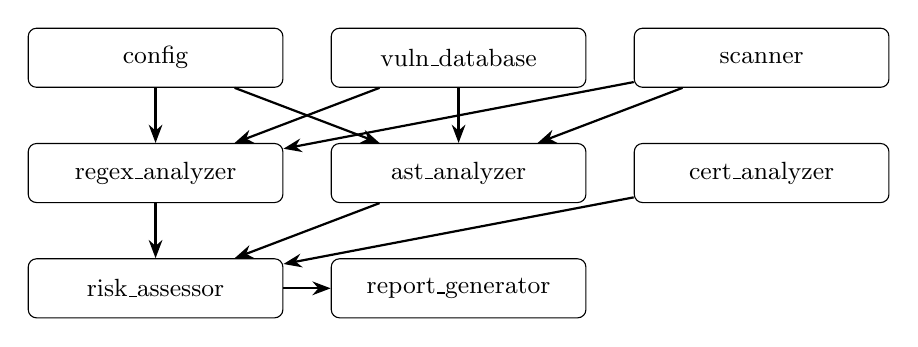
\begin{tikzpicture}[
  node distance=0.5cm and 0.4cm,
  mod/.style={rectangle, draw, rounded corners=3pt, text width=3.0cm, align=center, minimum height=0.75cm, font=\small},
  arr/.style={-Stealth, thick}
]
\node[mod] (cfg)    {config};
\node[mod, right=0.6cm of cfg] (db) {vuln\_database};
\node[mod, right=0.6cm of db]  (sc) {scanner};
\node[mod, below=0.7cm of cfg] (re) {regex\_analyzer};
\node[mod, right=0.6cm of re]  (ast){ast\_analyzer};
\node[mod, right=0.6cm of ast] (ca) {cert\_analyzer};
\node[mod, below=0.7cm of re]  (ra) {risk\_assessor};
\node[mod, right=0.6cm of ra]  (rg) {report\_generator};

\draw[arr] (cfg) -- (re); \draw[arr] (cfg) -- (ast);
\draw[arr] (db)  -- (re); \draw[arr] (db)  -- (ast);
\draw[arr] (sc)  -- (re); \draw[arr] (sc)  -- (ast);
\draw[arr] (re)  -- (ra); \draw[arr] (ast) -- (ra);
\draw[arr] (ca)  -- (ra); \draw[arr] (ra)  -- (rg);
\end{tikzpicture}
\caption{Компонентная архитектура инструмента}
\label{fig:structure}
\end{figure}

	Сам процесс обработки можно представить как последовательность вызовов (рисунок~\ref{fig:pipeline}). Сначала main.cpp вызывает разбор конфигурации. Затем загружается база уязвимостей. Далее выполняется сканирование проекта. После этого выбирается режим анализа кода: regex или AST. Затем при необходимости анализируются сертификаты. Далее выполняется оценка рисков. Последним этапом создаются отчеты.
	
	Внутренние структуры данных были спроектированы так, чтобы каждая из них соответствовала определенному уровню обработки. AppConfig описывает параметры запуска. ProjectInventory описывает структуру проекта. Finding описывает обнаруженный криптографический вызов. CertInfo описывает сертификат. RiskReport описывает результаты оценки риска. MigrationAction описывает одно действие плана миграции. Cbom описывает человекочитаемый криптографический инвентарь.
	
	AppConfig является конфигурационным объектом всего приложения. Он создается в самом начале работы из аргументов командной строки и далее передается тем модулям, которым нужны параметры запуска.
	
\begin{itmolisting}[C++]{Основные поля структуры AppConfig}{lst:appconfig-brief}
	struct AppConfig {
		std::string source_path;
		std::string cert_path;
		std::string db_path;
		std::string output_path;
		std::string cbom_output_path;
		AnalysisMode analysis_mode;
		bool verbose;
		bool cbom_only;
		bool skip_cert;
		bool run_metrics;
		std::string ground_truth_path;
		std::vector<std::string> extra_db_paths;
		std::vector<std::string> include_dirs;
	};
\end{itmolisting}
	
	Такое централизованное хранение параметров исключает ситуацию, когда отдельные модули самостоятельно читают аргументы командной строки. Это повышает связность конфигурации и делает поведение инструмента предсказуемым.

	
	
	
	Особенно важна структура Finding, поскольку она является связующим звеном между анализаторами, оценщиком риска и генератором отчетов. Она должна быть достаточно общей, чтобы подходить и для regex-режима, и для AST-режима. При этом она должна позволять AST-режиму передавать более подробные данные: класс, пространство имен и аргументы.
	
	Критически значимый фрагмент структуры Finding приведен в листинге~\ref{lst:finding}.

\begin{itmolisting}[C++]{Структура обнаружения Finding}{lst:finding}
	struct Finding {
		std::string file_path;
		std::string function_name;
		std::string library;
		std::string algorithm;
		std::string category;
		std::string quantum_vulnerability;
		
		std::string context_function;
		std::string context_class;
		std::string context_namespace;
		
		std::string raw_line;
		std::string analyzer_mode;
		std::string vuln_id;
		std::string nist_reference;
		std::string tc26_reference;
		
		int line_number;
		int column;
		double base_risk_score;
		
		std::vector<std::string> arguments;
	};
\end{itmolisting}
	
	Этот фрагмент важен для понимания всей архитектуры. Поля \textit{file\_path}, \textit{line\_number} и \textit{column} определяют место находки. Поля \textit{function\_name}, \textit{library}, \textit{algorithm} и \textit{category} описывают криптографическую сущность. Поля \textit{context\_function}, \textit{context\_class} и \textit{context\_namespace} делают результат объяснимым для разработчика. Поле \textit{base\_risk\_score} связывает находку с оценкой риска. Поле \textit{arguments} необходимо для более точного \textit{AST}-анализа, особенно для универсальных API OpenSSL.
	
	При проектировании также была заложена возможность расширения. Расширяемость реализуется на трех уровнях. Первый уровень -- база сигнатур: новые функции можно добавить в \textit{JSON}. Второй уровень -- языковые плагины: новые типы файлов можно добавить через реализацию \textit{ILanguagePlugin}. Третий уровень -- анализаторы: новый способ анализа можно добавить через реализацию интерфейса \textit{ICodeAnalyzer}.
	
	\section{Реализация инструмента}
	
	\subsection{Общая организация разработки}
	
	Проект реализован на C++17 и организован по классической схеме с разделением заголовочных файлов, исходных файлов, данных и тестов. Заголовочные файлы находятся в каталоге include/pqc, а реализации классов расположены в каталоге src. Данные базы уязвимых функций вынесены в отдельный JSON-файл. Тестовые данные и тесты размещены в каталоге tests.
	
	Общая структура проекта изображена на рисунке~\ref{fig:dir}.

\begin{figure}[htbp]
  \centering
  \small\ttfamily
  \begin{tabular}{@{}l@{\hspace{1cm}}l@{}}
    pqc-migration-tool/ & \\
    \quad{}├── include/pqc/ & \rmfamily\small --- заголовочные файлы (.hpp) \\
    \ttfamily\quad{}├── src/       & \rmfamily\small --- реализации классов (.cpp)  \\
    \ttfamily\quad{}├── data/      & \rmfamily\small --- база уязвимых функций (JSON)\\
    \ttfamily\quad{}└── tests/     & \\
    \ttfamily\quad{}\quad{}└── fixtures/ & \rmfamily\small --- тестовые данные и эталонная разметка \\
  \end{tabular}
  \caption{Структура каталогов проекта}
  \label{fig:dir}
\end{figure}

	Для сборки используется CMake версии не ниже 3.16. В проекте подключается библиотека nlohmann/json, OpenSSL и, при наличии, libclang. OpenSSL является обязательной зависимостью, поскольку без него невозможно выполнить анализ X.509-сертификатов. Libclang является опциональной зависимостью, так как режим регулярных выражений и токенный анализатор могут использоваться и без него.
	
	Внутренний поток данных показан на рисунке~\ref{fig:data-flow}.

\begin{figure}[htbp]
  \centering
  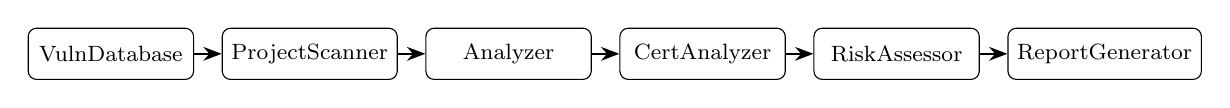
\begin{tikzpicture}[
    box/.style={draw, rounded corners=3pt, minimum width=2.1cm,
                minimum height=0.65cm, align=center, font=\footnotesize},
    arr/.style={-{Stealth}, thick},
    node distance=0.4cm and 0.35cm
  ]
    \node[box] (vd) {VulnDatabase};
    \node[box, right=of vd] (ps) {ProjectScanner};
    \node[box, right=of ps] (an) {Analyzer};
    \node[box, right=of an] (ca) {CertAnalyzer};
    \node[box, right=of ca] (ra) {RiskAssessor};
    \node[box, right=of ra] (rg) {ReportGenerator};
    \draw[arr] (vd) -- (ps);
    \draw[arr] (ps) -- (an);
    \draw[arr] (an) -- (ca);
    \draw[arr] (ca) -- (ra);
    \draw[arr] (ra) -- (rg);
  \end{tikzpicture}
  \caption{Внутренний поток данных конвейера}
  \label{fig:data-flow}
\end{figure}

	Важной особенностью реализации является то, что все ключевые результаты представлены как структуры данных, которые можно сериализовать в JSON. Это упрощает отладку, тестирование и последующую интеграцию инструмента в процессы непрерывного контроля безопасности.
	
	\subsection{Реализация конфигурации и командного интерфейса}
	
	Командный интерфейс реализован в модуле config.cpp и описан структурой AppConfig. Пользователь управляет работой инструмента через параметры запуска. Основным обязательным параметром является путь к анализируемому проекту.
	В таблице~\ref{tab:cli-impl} описаны основные параметры запуска.

	\begin{longtable}{|p{5.5cm}|p{10.0cm}|}
		% Заголовок подхватит стиль itmo автоматически из преамбулы
		\caption{Параметры и флаги командной строки} \label{tab:cli-impl} \\
		\hline
		Флаг & Описание \\ \hline
		\endfirsthead
		
		% Шапка на последующих страницах
		\multicolumn{2}{r}{\textit{Продолжение таблицы \thetable}} \\ \hline
		Флаг & Описание \\ \hline
		\endhead
		
		\hline
		\endlastfoot
		
		% Данные таблицы 
		\texttt{-s}, \texttt{--source <path>} & путь к исходному коду проекта \\ \hline
		\texttt{-c}, \texttt{--cert <path>} & путь к файлу или директории сертификатов \\ \hline
		\texttt{-d}, \texttt{--db <path>} & путь к JSON-базе уязвимых функций \\ \hline
		\texttt{-m}, \texttt{--mode <regex|ast>} & режим анализа кода \\ \hline
		\texttt{-I}, \texttt{--include <dir>} & include-директория для AST-анализа \\ \hline
		\texttt{-o}, \texttt{--output <path>} & путь к полному JSON-отчету \\ \hline
		\texttt{--cbom-output <path>} & путь к CBOM-отчету \\ \hline
		\texttt{--extra-db <path>} & дополнительная база сигнатур \\ \hline
		\texttt{--metrics} & включение расчета precision/recall/F1 \\ \hline
		\texttt{--ground-truth <path>} & файл эталонной разметки \\ \hline
		\texttt{--cbom-only} & генерация только CBOM \\ \hline
		\texttt{--skip-cert} & пропуск анализа сертификатов \\ \hline
		\texttt{-v}, \texttt{--verbose} & подробный режим вывода
	\end{longtable}
	
	
	Структура конфигурации приведена в листинге~\ref{lst:appconfig}: все параметры сведены в один объект, передаваемый через конвейер.

\begin{itmolisting}[C++]{Структура конфигурации AppConfig}{lst:appconfig}
struct AppConfig {
	std::string source_path;
	std::string cert_path;
	std::string db_path;
	std::string output_path;
	std::string cbom_output_path;
	AnalysisMode analysis_mode = AnalysisMode::REGEX;
	
	bool verbose = false;
	bool cbom_only = false;
	bool skip_cert = false;
	bool run_metrics = false;
	
	std::string ground_truth_path;
	std::vector<std::string> extra_db_paths;
	std::vector<std::string> include_dirs;
	
	static AppConfig parse(int argc, char** argv);
};
\end{itmolisting}

	Выбор режима анализа выполняется через перечисление AnalysisMode. Это исключает использование произвольных строковых значений во внутренних модулях и снижает вероятность ошибок. Строковые значения regex и ast используются только на границе программы, при разборе аргументов командной строки. После этого вся программа работает с типизированным значением.
	
	Причина выделения конфигурации в отдельный модуль состоит в том, что конфигурация затрагивает практически все последующие этапы. Например, db\_path нужен базе уязвимых функций, analysis\_mode нужен выбору анализатора, cert\_path и skip\_cert нужны модулю сертификатов, а ground\_truth\_path нужен модулю метрик. Если бы разбор аргументов был распределен по разным частям программы, поддерживать согласованность стало бы намного сложнее.
	
	\subsection{Реализация базы уязвимых функций}
	
	База уязвимых функций является одним из центральных элементов инструмента. Она хранится в файле data/vulnerable\_functions.json и загружается классом VulnDatabase. В текущей реализации база имеет версию 2.0 и включает функции из нескольких групп библиотек: OpenSSL, Crypto++ и реализации ГОСТ-алгоритмов.
	
	Содержательно база была сформирована как перечень криптографических API, использование которых указывает на применение алгоритмов, потенциально уязвимых к квантовым атакам или уже признанных устаревшими. В нее включены алгоритмы RSA, DSA, DH, ECDH, ECDSA, отдельные EVP-вызовы OpenSSL, низкоуровневые структуры ключей, а также устаревшие хэш-функции. Отдельно включены функции и обозначения для ГОСТ-алгоритмов, поскольку при разработке учитывалась не только международная, но и российская криптографическая практика.
	
	Структура JSON-записи базы данных приведена в листинге~\ref{lst:bd}.

\begin{itmolisting}[JSON]{Пример JSON-записи базы уязвимых функций}{lst:bd}
{
	"id": "openssl-rsa-keygen",
	"name": "RSA_generate_key",
	"library_name": "openssl",
	"category": "asymmetric_encryption",
	"algorithm": "RSA",
	"quantum_vulnerability": "Shor algorithm",
	"risk_score": 10.0,
	"aliases": ["RSA_generate_key_ex"],
	"patterns": ["\\bRSA_generate_key\\s*\\(", "\\bRSA_generate_key_ex\\s*\\("],
	"context_keywords": ["key", "certificate", "tls"],
	"nist_reference": "NIST PQC migration recommendations",
	"tc26_reference": "TC26 migration note",
	"replacements": [
	{
		"function_name": "ML-KEM",
		"library": "OpenSSL provider or PQC library",
		"standard": "FIPS 203",
		"algorithm": "ML-KEM",
		"type": "key_encapsulation",
		"migration_notes": "Replace RSA key transport with KEM-based or hybrid scheme",
		"example_code": "...",
		"tc26_note": "Consider national regulatory requirements"
	}
	]
}
\end{itmolisting}

В реальном файле база содержит не одну запись, а набор записей для разных библиотек и алгоритмов. Группы функций, относящихся к OpenSSL, представлены в таблице~\ref{tab:openssl}.

\begin{longtable}{|l|p{5.0cm}|p{6.5cm}|}
	% Заголовок подхватит стиль itmo автоматически из преамбулы
	\caption{Классификация функций криптографических библиотек для миграции} \label{tab:openssl} \\
	\hline
	Группа & Примеры функций & Причина включения \\ \hline
	\endfirsthead
	
	% Шапка на последующих страницах
	\multicolumn{3}{r}{\textit{Продолжение таблицы \thetable}} \\ \hline
	Группа & Примеры функций & Причина включения \\ \hline
	\endhead
	\hline
	\endlastfoot
	
	% Данные таблицы (ширина колонок подобрана, чтобы текст не вылезал за поля)
	RSA & \texttt{RSA\_generate\_key}, \texttt{RSA\_generate\_key\_ex}, \texttt{RSA\_public\_encrypt}, \texttt{RSA\_private\_decrypt}, \texttt{RSA\_sign}, \texttt{RSA\_verify} & RSA уязвим к квантовой атаке на факторизацию. \\ \hline
	DSA & \texttt{DSA\_sign}, \texttt{DSA\_verify}, \texttt{DSA\_do\_sign}, \texttt{DSA\_do\_verify} & DSA основан на сложности дискретного логарифмирования. \\ \hline
	DH & \texttt{DH\_generate\_key}, \texttt{DH\_compute\_key} & Классический Диффи-Хеллман уязвим при наличии квантового компьютера. \\ \hline
	ECDH & \texttt{ECDH\_compute\_key} & Эллиптический Диффи-Хеллман также относится к уязвимым схемам. \\ \hline
	ECDSA & \texttt{ECDSA\_sign}, \texttt{ECDSA\_verify}, \texttt{ECDSA\_do\_sign}, \texttt{ECDSA\_do\_verify} & Подпись на эллиптических кривых уязвима к квантовой атаке. \\ \hline
	EVP & \texttt{EVP\_PKEY\_encrypt}, \texttt{EVP\_PKEY\_decrypt}, \texttt{EVP\_DigestSignInit}, \texttt{EVP\_PKEY\_CTX\_new} & Высокоуровневые вызовы OpenSSL могут скрывать RSA, ECDSA, DH и другие алгоритмы. \\ \hline
	BIGNUM & отдельные операции \texttt{BN\_*} & Могут быть признаком ручной реализации криптографических примитивов. \\ \hline
	Устаревшие хэши & \texttt{SHA1}, \texttt{MD5} & Не являются основной целью постквантовой миграции, но важны для общей криптографической инвентаризации.
\end{longtable}


Классы и типы, характерные для библиотеки Crypto++, указаны в таблице~\ref{tab:crypto}.

\begin{longtable}{|p{6.7cm}|p{6.6cm}|l|}
	% Заголовок подхватит стиль itmo автоматически из преамбулы
	\caption{Классификация объектов библиотеки Crypto++ по уровням риска} \label{tab:crypto} \\
	\hline
	Запись & Псевдонимы & Риск \\ \hline
	\endfirsthead
	
	% Шапка на последующих страницах
	\multicolumn{3}{r}{\textit{Продолжение таблицы \thetable}} \\ \hline
	Запись & Псевдонимы & Риск \\ \hline
	\endhead
	
	\hline
	\endlastfoot
	
	% Данные таблицы (моноширинный текст обернут в \texttt для правильного отображения кода)
	\texttt{RSA::PrivateKey} & \texttt{RSA::PublicKey}, \texttt{InvertibleRSAFunction} & Высокий \\ \hline
	\texttt{RSAES\_OAEP\_SHA\_Encryptor} & \texttt{RSAES\_PKCS1v15\_Encryptor}, \texttt{RSAES\_OAEP\_SHA\_Decryptor} & Высокий \\ \hline
	\texttt{ECDH} & \texttt{ECMQV} & Высокий \\ \hline
	\texttt{ECDSA} & \texttt{ECGDSA}, \texttt{ECNR} & Высокий \\ \hline
	\texttt{DH2} & \texttt{DH}, \texttt{MQV} & Высокий
\end{longtable}


Для ГОСТ-направления включены записи gost\_ec\_sign, gost\_ec\_verify, GOST\_R3410\_keypair, VKO\_cryptopro\_2001, VKO\_cryptopro\_2012, gost\_vko\_compute. Их включение важно, поскольку инструмент должен быть применим не только к проектам, использующим OpenSSL, но и к коду, в котором встречаются национальные криптографические механизмы.

Класс VulnDatabase отвечает за загрузку базы, объединение основной и дополнительных баз, построение индекса имён и поиск функций. Его интерфейс приведён в листинге~\ref{lst:vulndb-class}.

\begin{itmolisting}[C++]{Интерфейс класса VulnDatabase}{lst:vulndb-class}
	class VulnDatabase {
		public:
		bool load(const std::string& path);
		bool merge_json(const nlohmann::json& j);
		
		const VulnerableFunction* find_by_name(
		const std::string& name
		) const;
		
		const std::vector<VulnerableFunction>& all() const;
		std::vector<VulnerableFunction> by_library(
		const std::string& library
		) const;
		
		std::string db_version() const;
		std::string last_updated() const;
		std::size_t size() const;
		
		private:
		std::vector<VulnerableFunction> functions_;
		std::unordered_map<std::string, std::size_t> name_index_;
		
		void rebuild_index();
		static std::string to_lower(std::string s);
	};
\end{itmolisting}

Ключевой технический момент состоит в методе rebuild\_index. После загрузки база строит индекс по имени функции и по всем псевдонимам. Поиск выполняется без учета регистра. Это позволяет анализатору не перебирать весь массив функций при каждой находке, а быстро получать описание уязвимой функции по имени.

Такое решение также позволяет подключать дополнительные базы через параметр --extra-db. Например, если организация использует собственную криптографическую обертку CompanyRSAEncrypt, ее можно добавить во внешний JSON-файл, не изменяя исходный код анализатора.

\subsection{Реализация инвентаризации проекта}

Инвентаризация проекта реализована классом ProjectScanner. Ее задача состоит в том, чтобы до запуска анализа получить полную картину состава проекта. Это необходимо по двум причинам. Во-первых, анализаторы должны получать только релевантные файлы. Во-вторых, контекст файла влияет на риск: тестовый код, сетевой код и код хранения данных должны интерпретироваться по-разному.

Для классификации файлов используется расширяемая система языковых плагинов, описанная в листинге~\ref{lst:inv}.

\begin{itmolisting}[C++]{Интерфейс языкового плагина ILanguagePlugin}{lst:inv}
class ILanguagePlugin {
	public:
	virtual ~ILanguagePlugin() = default;
	
	virtual std::string language_name() const = 0;
	
	virtual bool matches(
	const std::filesystem::path& path
	) const = 0;
	
	virtual FileCategory categorize(
	const std::filesystem::path& path
	) const = 0;
};
\end{itmolisting}

В текущей реализации предусмотрены плагины для C/C++-файлов, CMake-файлов и сертификатов. Плагин C++ распознает исходные и заголовочные файлы по расширениям. Плагин CMake относит CMakeLists.txt и похожие файлы к сборочным. Плагин сертификатов определяет файлы сертификатов по расширениям, характерным для PEM, CRT, CER и DER. Фрагмент логики сканирования описан в листинге~\ref{lst:inv2}.

\begin{itmolisting}[C++]{Метод сканирования ProjectScanner}{lst:inv2}
	ProjectInventory ProjectScanner::scan(
	const std::string& root_path
	) const {
		ProjectInventory inventory;
		inventory.project_path = root_path;
		inventory.project_name =
		std::filesystem::path(root_path).filename().string();
		
		for (const auto& entry :
		std::filesystem::recursive_directory_iterator(root_path)) {
			if (!entry.is_regular_file()) {
				continue;
			}
			
			if (should_skip(entry.path())) {
				continue;
			}
			
			FileEntry file;
			file.path = entry.path().string();
			file.size_bytes = entry.file_size();
			file.category = detect_category(entry.path());
			file.language = detect_language(entry.path());
			file.line_count = count_lines(entry.path());
			
			inventory.files.push_back(file);
			inventory.language_stats[file.language]++;
		}
		
		return inventory;
	}
\end{itmolisting}

В реальном коде сканер также исключает служебные каталоги. Это важно, потому что анализ каталогов сборки, зависимостей или истории Git увеличил бы число ложных срабатываний и замедлил бы работу. Например, каталог build может содержать сгенерированные файлы, а .git содержит служебные объекты, которые не должны рассматриваться как исходный код проекта.

Результатом сканирования является ProjectInventory. Он может быть выведен в виде сводки, использован для выбора файлов анализа и преобразован в метаданные CBOM. Например, если проект содержит 200 файлов, но только 35 из них относятся к исходному коду C++, анализаторы получают именно эти 35 файлов, а не документацию, изображения или служебные ресурсы.

Внутренняя логика инвентаризации схематично представлена на рисунке~\ref{fig:inv}.

\begin{figure}[htbp]
  \centering
  \begin{tikzpicture}[
    block/.style={draw, rounded corners=3pt, minimum width=4.5cm,
                  minimum height=0.65cm, align=center, font=\small},
    decision/.style={draw, diamond, aspect=2.5, font=\small, align=center},
    arr/.style={-{Stealth}, thick},
    node distance=0.5cm
  ]
    \node[block] (scan)  {Рекурсивный обход директории};
    \node[block, below=of scan]  (skip)  {Проверка исключений};
    \node[decision, below=of skip] (dec) {Пропустить?};
    \node[block,  below=of dec]  (cat)   {Определение категории и языка};
    \node[block,  below=of cat]  (add)   {Добавление FileEntry в инвентарь};
    \node[block,  below=of add]  (ret)   {Возврат ProjectInventory};
    \node[right=1.5cm of dec, font=\small] (skip2) {следующий файл};

    \draw[arr] (scan) -- (skip);
    \draw[arr] (skip) -- (dec);
    \draw[arr] (dec)  -- node[right,font=\small]{Нет} (cat);
    \draw[arr] (dec)  -- node[above,font=\small]{Да} (skip2);
    \draw[arr] (cat)  -- (add);
    \draw[arr] (add)  -- (ret);
  \end{tikzpicture}
  \caption{Логика инвентаризации проекта}
  \label{fig:inv}
\end{figure}

Главное преимущество такой схемы заключается в том, что добавление нового типа файлов не требует переписывания сканера. Достаточно реализовать новый плагин, который сможет проанализировать файл и определить его категорию.


\subsection{Реализация общего интерфейса анализаторов}

Общий интерфейс анализаторов введен для того, чтобы разные методы статического анализа могли быть взаимозаменяемыми. В проекте реализованы три подхода: анализ регулярными выражениями, анализ на уровне токенов и AST. Объявление самого интерфейса описано в листинге~\ref{lst:analyzer}.

\begin{itmolisting}[C++]{Интерфейс анализатора кода ICodeAnalyzer}{lst:analyzer}
class ICodeAnalyzer {
	public:
	virtual ~ICodeAnalyzer() = default;
	
	virtual std::string mode_name() const = 0;
	
	virtual std::vector<Finding> analyze(
	const ProjectInventory& inventory,
	const VulnDatabase& db
	) = 0;
	
	virtual std::vector<Finding> analyze_file(
	const FileEntry& file,
	const VulnDatabase& db
	) = 0;
};
\end{itmolisting}

Метод analyze работает с полной инвентаризацией проекта, а analyze\_file анализирует один файл. Такое разделение удобно для тестирования: модульные тесты могут проверять отдельный файл, а интеграционные тесты могут проверять полный конвейер.

Единый интерфейс также позволяет сравнивать разные режимы анализа на одинаковых тестовых данных. Например, один и тот же файл sample\_vulnerable.cpp может быть передан RegexAnalyzer и ASTAnalyzer, после чего результаты сравниваются с эталонной разметкой.

Важно отметить, что все результаты имеют общий формат, который в дальнейшем передается на вход модулю оценки риска. С точки зрения архитектуры это решение является принципиально важным: если в будущем будет добавлен анализатор для Python, Java или Go, он также сможет возвращать Finding, а остальные этапы останутся без изменений.

\subsection{Реализация анализатора регулярных выражений}

Анализатор регулярных выражений реализован в классе RegexAnalyzer. Он является самым простым и быстрым из режимов анализа. Его задача: построчно прочитать исходный файл и найти в нем вызовы функций, описанных в базе уязвимых функций.

Для каждой функции из базы используется два источника шаблонов: явно заданные регулярные выражения из поля patterns и автоматически сформированный шаблон. Это позволяет находить вызовы, даже если для функции не задан отдельный шаблон. Принцип его работы представлен в листинге~\ref{lst:regex}.

	
\begin{itmolisting}[C++]{Основной цикл сопоставления паттернов RegexAnalyzer}{lst:regex}
for (const auto& vf : db.all()) {
	std::vector<std::regex> compiled_patterns;
	
	for (const auto& pattern : vf.patterns) {
		compiled_patterns.emplace_back(pattern);
	}
	
	std::string auto_pattern =
	"\\b" + escape_regex(vf.name) + "\\s*\\(";
	compiled_patterns.emplace_back(auto_pattern);
	
	for (const auto& re : compiled_patterns) {
		auto begin = std::sregex_iterator(
		line.begin(), line.end(), re
		);
		auto end = std::sregex_iterator();
		
		for (auto it = begin; it != end; ++it) {
			Finding finding;
			finding.file_path = file.path;
			finding.function_name = vf.name;
			finding.library = vf.library_name;
			finding.algorithm = vf.algorithm;
			finding.category = vf.category;
			finding.quantum_vulnerability =
			vf.quantum_vulnerability;
			finding.line_number = line_number;
			finding.column = static_cast<unsigned>(
			it->position() + 1
			);
			finding.raw_line = line;
			finding.analyzer_mode = mode_name();
			finding.vuln_id = vf.id;
			finding.base_risk_score = vf.risk_score;
			
			out.push_back(finding);
		}
	}
}
\end{itmolisting}

На практике в реализации также используется дедупликация по имени функции и номеру строки. Это необходимо, потому что одна и та же функция может быть найдена одновременно по явному шаблону и по автоматически построенному шаблону. Без дедупликации отчет содержал бы повторяющиеся находки, что исказило бы оценку риска и расчет нужных метрик.

У анализатора регулярных выражений есть важное достоинство: он быстро работает и не требует внешних зависимостей, кроме стандартной библиотеки C++. Его можно использовать для первичной оценки проекта и для окружений, где недоступен libclang.

Однако у этого режима есть и ограничения. Регулярное выражение анализирует текст, а не структуру программы. Поэтому оно может сработать на строковом литерале, многострочном комментарии или макросе. В текущей реализации частично учитываются однострочные комментарии, но полноценное понимание синтаксиса C++ в этом режиме не выполняется. Именно для борьбы с этой проблемой и был реализован анализатор на уровне AST.

\subsection{Реализация AST-анализатора}

AST-анализатор является наиболее сложным компонентом инструмента. Он реализован в классе ASTAnalyzer и использует libclang для построения абстрактного синтаксического дерева C++-кода. В отличие от регулярных выражений и токенов, AST-анализатор работает не только с текстом, но и со структурой программы: функциями, методами, классами, вызовами, аргументами, локальными переменными и областями видимости.

\subsubsection{Парсинг единицы трансляции}
	
Для каждого анализируемого исходного файла создается своя единица трансляции. Помимо стандартных параметров в libclang также передаются пути к include-директориям, указанным пользователям.

Концептуально этот этап выглядит так (листинг~\ref{lst:ast-stage1}):

\begin{itmolisting}[C++]{Параметры разбора единицы трансляции через libclang}{lst:ast-stage1}
const char* args[] = {
	"-x", "c++",
	"-std=c++17",
	"-w",
	"-ferror-limit=0"
};

CXTranslationUnit tu = clang_parseTranslationUnit(
	index,
	file.path.c_str(),
	args,
	arg_count,
	nullptr,
	0,
	CXTranslationUnit_DetailedPreprocessingRecord |
	CXTranslationUnit_KeepGoing
);
\end{itmolisting}

Последний флаг (игнорирование некритичных ошибок) очень важен для практического анализа. В реальных проектах отдельный файл может не разбираться идеально из-за отсутствующих зависимостей или специфических флагов сборки. Задача инструмента не состоит в полной компиляции проекта, поэтому анализатор должен по возможности продолжать работу даже при наличии ошибок разбора.


\subsubsection{Построение внутренней модели функций}

Первая фаза ASTAnalyzer собирает сведения обо всех определенных функциях, методах, конструкторах и деструкторах. Для каждой функции создается свой FunctionSummary (листинг~\ref{lst:ast-stage2}):

\begin{itmolisting}[C++]{Структура сводки функции FunctionSummary}{lst:ast-stage2}
struct FunctionSummary {
	std::string qualified_name;
	std::string simple_name;
	std::string file_path;
	
	CXCursor cursor{};
	bool has_cursor = false;
	
	bool is_static = false;
	bool in_anon_ns = false;
	bool is_definition = false;
	
	std::vector<std::string> param_names;
	std::vector<std::string> param_types;
	
	std::unordered_map<std::string, std::vector<LocalValue>> locals;
	
	CXCursor return_cursor{};
	bool has_return_cursor = false;
	
	std::vector<std::string> callees;
};
\end{itmolisting}

Эта структура показывает, что анализатор строит не просто список вызовов, а внутреннюю модель функций. qualified\_name нужен для различения функций в разных классах и пространствах имен; simple\_name нужен для сопоставлений по имени; param\_names и param\_types нужны для разрешения аргументов; locals хранит историю локальных переменных; callees используется для построения графа вызовов.

\subsubsection{Сбор локальных значений}

На второй фазе анализатор заполняет тела функций. Одной из ключевых задач является сбор значений локальных переменных. Для этого используется структура LocalValue (листинг~\ref{lst:ast-stage31}):

\begin{itmolisting}[C++]{Структура значения локальной переменной}{lst:ast-stage31}
struct LocalValue {
	std::string text;
	unsigned line = 0;
	bool known = false;
};
\end{itmolisting}

Значения хранятся как история, а не как одно последнее значение. Это позволяет учитывать переопределения переменной. Если переменная имеет несколько присваиваний, при разрешении аргумента выбирается то значение, которое было актуально до строки вызова.

Пример ситуации, для которой нужен такой механизм, приведен в листинге~\ref{lst:ast-stage32}.

\begin{itmolisting}[C++]{Пример отслеживания аргумента через локальную переменную}{lst:ast-stage32}
	const char* alg = "RSA";
	EVP_PKEY_CTX* ctx = EVP_PKEY_CTX_new_from_name(nullptr, alg, nullptr);
\end{itmolisting}

Анализатор на основе регулярных выражений в такой ситуации увидит только вызов EVP\_PKEY\_CTX\_new\_from\_name. AST-анализатор может попытаться понять, что аргумент alg соответствует строке "RSA". Это особенно важно для универсальных EVP-функций OpenSSL, где реальный алгоритм передается параметром.

\subsubsection{Сбор полей классов и побочных эффектов}

Особенность C++-кода состоит в том, что криптографические объекты часто хранятся в полях классов, а операции с ними выполняются в разных методах. Поэтому в AST-анализаторе реализованы дополнительные фазы сбора полей классов и эффектов методов.

Сведения о полях позволяют анализатору понимать, что объект, созданный или записанный в одном методе, может использоваться в другом. Для этого также используется структура событий метода (листинг~\ref{lst:ast-stage4}).

\begin{itmolisting}[C++]{Структуры полей класса и событий метода}{lst:ast-stage4}
struct FieldInfo {
	std::string type_spelling;
	std::string resolved_value;
	bool has_value = false;
};

struct MethodEvent {
	enum class Kind {
		Mutation,
		IntraClassCall
	};
	
	Kind kind;
	unsigned line = 0;
	std::string mutation;
	std::string call_qualified;
};
\end{itmolisting}

Событие Mutation означает изменение состояния объекта, а IntraClassCall означает вызов другого метода того же класса. Это нужно для восстановления точной последовательности действий внутри объектно-ориентированного кода.
	
\subsubsection{Построение достижимости}

После сбора функций и их вызовов ASTAnalyzer вычисляет достижимость. Корнями считаются main и функции с внешней линковкой, то есть функции, которые потенциально могут вызываться извне translation unit. Далее выполняется BFS по графу вызовов.

Недостижимые функции не исключаются из отчета полностью. Вместо этого для них применяется понижающий коэффициент риска (листинг~\ref{lst:ast-stage5}).

\begin{itmolisting}[C++]{Коэффициент риска для недостижимых функций}{lst:ast-stage5}
static constexpr double kUnreachableRiskFactor = 0.3;

f.base_risk_score = pc.reachable_from_root
? opt->risk_score
: opt->risk_score * kUnreachableRiskFactor;
\end{itmolisting}

Это важное проектное решение. Если полностью исключить недостижимые функции, можно пропустить реальный риск, потому что анализ выполняется в пределах одной translation unit и может не видеть внешние точки входа. Если же не учитывать достижимость вообще, то мертвый или вспомогательный код будет получать такой же приоритет, как реально исполняемый. Использование коэффициента 0.3 является компромиссом: находка сохраняется, но ее приоритет заметно снижается.

\subsubsection{Разрешение аргументов}

Одна из наиболее важных возможностей AST-анализатора -- разрешение аргументов вызова. Для этого используется ResolutionContext (листинг~\ref{lst:ast-stage6}), который объединяет текущий фрейм функции, сводки функций, привязки параметров, реестр полей класса и динамическое состояние полей.

	
\begin{itmolisting}[C++]{Контекст разрешения аргументов ResolutionContext}{lst:ast-stage6}
	struct ResolutionContext {
		FunctionFrame* frame;
		
		const std::unordered_map<std::string, FunctionSummary>* summaries;
		
		std::unordered_map<std::string, std::string> param_bindings;
		
		std::unordered_set<std::string> active_functions;
		
		const ClassFieldRegistry* field_registry;
		
		std::string current_class_qualified;
		std::string current_class_simple;
		
		const FieldStateMap* dynamic_field_state;
	};
\end{itmolisting}

Схема процесса разрешения аргумента представлена на рисунке~\ref{fig:arg}.

\begin{figure}[h]
\centering
\begin{tikzpicture}[
  node distance=1.2cm and 0.6cm,
  box/.style={rectangle, draw, rounded corners=3pt, text width=3.5cm, align=center, minimum height=0.8cm, font=\small},
  decision/.style={diamond, draw, aspect=2.5, text width=3.2cm, align=center, font=\small},
  arr/.style={-Stealth, thick}
]
\node[box] (start) {Аргумент вызова};
\node[decision, below=of start] (d1) {Строковой литерал?};
\node[box, right=2.2cm of d1] (ret1) {Вернуть значение напрямую};
\node[decision, below=of d1] (d2) {Локальная переменная?};
\node[box, right=2.2cm of d2] (ret2) {Взять последнее значение из истории};
\node[decision, below=of d2] (d3) {Параметр функции?};
\node[box, right=2.2cm of d3] (ret3) {Взять из param\_bindings};
\node[decision, below=of d3] (d4) {Поле класса?};
\node[box, right=2.2cm of d4] (ret4) {Взять из dynamic\_field\_state};
\node[box, below=of d4] (unresp) {Значение не разрешено};

\draw[arr] (start) -- (d1);
\draw[arr] (d1) -- node[above,font=\small]{да} (ret1);
\draw[arr] (d1) -- node[left,font=\small]{нет} (d2);
\draw[arr] (d2) -- node[above,font=\small]{да} (ret2);
\draw[arr] (d2) -- node[left,font=\small]{нет} (d3);
\draw[arr] (d3) -- node[above,font=\small]{да} (ret3);
\draw[arr] (d3) -- node[left,font=\small]{нет} (d4);
\draw[arr] (d4) -- node[above,font=\small]{да} (ret4);
\draw[arr] (d4) -- node[left,font=\small]{нет} (unresp);
\end{tikzpicture}
\caption{Схема разрешения аргумента вызова в AST-анализаторе}
\label{fig:arg}
\end{figure}

Такой механизм особенно важен для вызовов вида EVP\_PKEY\_CTX\_new\_from\_name. В этом случае сама функция является универсальной, а конкретный алгоритм определяется строковым аргументом. Если ASTAnalyzer может разрешить этот аргумент, отчет становится существенно точнее.

\subsubsection{Ограничения AST-анализатора}

Несмотря на большую глубину анализа, AST-анализатор имеет значительные ограничения. Он анализирует единицы трансляции отдельно и не выполняет полноценный межмодульный анализ. Заголовочные файлы не анализируются как самостоятельные файлы с исходным кодом, хотя могут попадать в анализ через механизм включения. Вызовы через указатели на функции не разрешаются полностью. Глубина разрешения выражений, подстановки функций и обхода графа вызовов ограничена константами (листинг~\ref{lst:ast-stage7}):

\begin{itmolisting}[C++]{Константы глубины анализа}{lst:ast-stage7}
static constexpr int kMaxResolveDepth = 12;
static constexpr int kMaxInlineExpansionDepth = 6;
static constexpr int kMaxCallGraphDepth = 8;
static constexpr std::size_t kMaxResolvedText = 512;
\end{itmolisting}

Эти ограничения необходимы для предотвращения бесконечной рекурсии и чрезмерного роста времени анализа. Они также задают границы применимости инструмента: AST-анализатор повышает точность по сравнению с регулярными выражениями, но не является полноценным компиляторным анализатором всех возможных путей выполнения.

\subsection{Реализация анализа сертификатов}

Модуль CertAnalyzer анализирует X.509-сертификаты как отдельный тип криптографических активов. Это важно, поскольку проект может содержать сертификаты, даже если соответствующие криптографические операции в исходном коде не отражены явно.

Алгоритм анализа сертификата состоит из нескольких этапов (рисунок~\ref{fig:cert-a}). Сначала файл открывается и анализатор пытается прочитать его как PEM. Если PEM-чтение не удалось, выполняется попытка чтения DER. Такой порядок выбран потому, что PEM часто используется в репозиториях и может содержать цепочку сертификатов, а DER представляет бинарный формат одного сертификата.

\begin{figure}[h]
\centering
\begin{tikzpicture}[
  node distance=1.1cm and 0.5cm,
  box/.style={rectangle, draw, rounded corners=3pt, text width=3.8cm, align=center, minimum height=0.75cm, font=\small},
  decision/.style={diamond, draw, aspect=2.6, text width=3.2cm, align=center, font=\small},
  arr/.style={-Stealth, thick}
]
\node[box] (open)  {Открыть файл};
\node[decision, below=of open]  (pem)   {Чтение PEM\\успешно?};
\node[box, right=2.4cm of pem] (chain) {Обработать цепочку\\сертификатов};
\node[decision, below=of pem]   (der)   {Чтение DER\\успешно?};
\node[box, right=2.4cm of der] (single){Обработать один\\сертификат};
\node[box, below=of der]       (skip)  {Файл пропущен};
\node[box, below=3.6cm of pem, xshift=2.4cm] (extract) {Извлечь атрибуты:\\алгоритм, размер ключа,\\даты, подпись};
\node[box, below=of extract]   (risk)  {Вычислить квантовый\\риск сертификата};

\draw[arr] (open)  -- (pem);
\draw[arr] (pem)   -- node[above,font=\small]{да}  (chain);
\draw[arr] (pem)   -- node[left,font=\small]{нет}  (der);
\draw[arr] (der)   -- node[above,font=\small]{да}  (single);
\draw[arr] (der)   -- node[left,font=\small]{нет}  (skip);
\draw[arr] (chain) -- (extract);
\draw[arr] (single) -- (extract);
\draw[arr] (extract)-- (risk);
\end{tikzpicture}
\caption{Алгоритм чтения и анализа сертификата}
\label{fig:cert-a}
\end{figure}

Ключевые операции извлечения данных выполняются через OpenSSL API (листинг~\ref{lst:cert-lib}):

\begin{itmolisting}[C++]{Вызовы OpenSSL API при разборе сертификата}{lst:cert-lib}
X509_NAME_print_ex(...);
ASN1_INTEGER_to_BN(...);
BN_bn2hex(...);
ASN1_TIME_print(...);
ASN1_TIME_diff(...);
X509_get0_signature(...);
X509_get0_pubkey(...);
EVP_PKEY_base_id(...);
EVP_PKEY_bits(...);
\end{itmolisting}

Оценка квантового риска сертификата выполняется по алгоритму открытого ключа и алгоритму подписи. RSA, ECDSA, ECDH, DSA, EC, Ed25519, Ed448 и ГОСТ классифицируются как высокий риск в рамках постквантовой модели. MD5 также получает высокий риск, но по причине классической криптографической слабости. SHA-1 получает средний риск. SHA-384 и SHA-512 получают низкий риск.

Численная оценка риска сертификата вычисляется по формуле:
\begin{equation}
\label{eq:cert-risk}
R_{cert} = \min\!\left(10{,}0;\; s_{base}(qr) + \delta_{rsa} - \delta_{exp}\right),
\end{equation}
где $s_{base}$ принимает значения $9{,}0$ при высоком квантовом риске, $5{,}5$ при среднем и $2{,}0$ при низком; $\delta_{rsa} = 0{,}5$ при алгоритме RSA с длиной ключа менее 2048 бит, иначе $0$; $\delta_{exp} = 1{,}0$ для просроченного сертификата, иначе $0$.

Уменьшение риска для просроченного сертификата связано с тем, что такой сертификат, как правило, уже не должен использоваться в активной инфраструктуре. Однако он все равно сохраняется в отчете, потому что может быть частью тестовой среды или legacy-конфигурации.

Ограничение модуля состоит в том, что он не проверяет цепочку доверия и не выполняет полную TLS-валидацию. Его задача - инвентаризация и классификация сертификатов как криптографических активов, а не проверка корректности PKI.
	
\subsection{Реализация оценки рисков}

Оценка риска реализована в классе RiskAssessor. Он получает на вход список находок, инвентаризацию проекта и список сертификатов. Результатом является RiskReport, содержащий общий риск, распределение по приоритетам, файловые сводки и план миграции.

Главная идея модуля: базовая опасность алгоритма должна корректироваться контекстом. Например, RSA\_sign в тестовом файле и RSA\_sign в модуле подписи производственных данных не должны иметь одинаковый итоговый приоритет. Контекст описывается структурой ContextFactors (листинг~\ref{lst:risk-context}).

\begin{itmolisting}[C++]{Структура контекстных факторов ContextFactors}{lst:risk-context}
struct ContextFactors {
	bool is_network_facing = false;
	bool is_persistent_data = false;
	bool is_key_material = false;
	bool is_in_loop = false;
	bool is_test_code = false;
	
	int call_frequency = 1;
	std::string data_classification;
};
\end{itmolisting}

В контексте данной реализации используются следующие множители (таблица~\ref{tab:factors}):

\begin{longtable}{|p{4cm}|p{3cm}|p{8cm}|}
	% Заголовок подхватит стиль itmo автоматически из преамбулы
	\caption{Коэффициенты корректировки риска по факторам кода} \label{tab:factors} \\
	\hline
	Фактор & Множитель & Интерпретация \\ \hline
	
	% Данные таблицы 
	\hspace{0pt}Тестовый код & 0.70 & \hspace{0pt}Риск снижается, так как код не относится к рабочему контуру. \\ \hline
	\hspace{0pt}Сетевой модуль & 1.30 & \hspace{0pt}Риск повышается из-за возможного внешнего воздействия. \\ \hline
	\hspace{0pt}Постоянно хранимые данные & 1.25 & \hspace{0pt}Риск повышается из-за долговременной ценности данных. \\ \hline
	\hspace{0pt}Ключевой материал & 1.20 & \hspace{0pt}Риск повышается при работе с ключами. \\ \hline
	\hspace{0pt}Вызов в цикле & 1.10 & \hspace{0pt}Риск повышается из-за частоты использования. \\ \hline
	\hspace{0pt}Частота вызова больше 5 & 1.10 & \hspace{0pt}Риск повышается при многократном использовании функции. \\
	\hline
\end{longtable}

Итоговая формула риска описана в листинге~\ref{lst:final-score}.


\begin{itmolisting}[C++]{Формула риска}{lst:final-score}
final_score = min(10.0, base_score * context_multiplier)
\end{itmolisting}


Фрагмент самой логики расчета представляется так (листинг~\ref{lst:risk-logic}):

	
\begin{itmolisting}[C++]{Метод вычисления оценки риска compute\_risk}{lst:risk-logic}
RiskScore RiskAssessor::compute_risk(
const Finding& finding,
const ContextFactors& factors
) const {
	double multiplier = 1.0;
	
	if (factors.is_test_code) {
		multiplier *= 0.70;
	}
	if (factors.is_network_facing) {
		multiplier *= 1.30;
	}
	if (factors.is_persistent_data) {
		multiplier *= 1.25;
	}
	if (factors.is_key_material) {
		multiplier *= 1.20;
	}
	if (factors.is_in_loop) {
		multiplier *= 1.10;
	}
	if (factors.call_frequency > 5) {
		multiplier *= 1.10;
	}
	
	RiskScore score;
	score.base_score = finding.base_risk_score;
	score.context_multiplier = multiplier;
	score.final_score =
	std::min(10.0, score.base_score * multiplier);
	score.priority = priority_for(score.final_score);
	score.factors = factors;
	
	return score;
}
\end{itmolisting}


Кроме отдельных находок, RiskAssessor формирует агрегированные данные по файлам. Для каждого файла сохраняются количество находок, максимальный риск, средний риск, общий приоритет и список имен функций. Это помогает понять, какие файлы являются наиболее проблемными с точки зрения предстоящей миграции.

Общий риск проекта рассчитывается как среднее значение по наиболее значимым находкам, а затем корректируется с учетом максимального риска сертификатов. В текущей реализации сертификаты влияют на итоговую оценку с весом 0.3, а находки в коде с весом 0.7 (листинг~\ref{lst:final-risk}).

\begin{itmolisting}[C++]{Формула итогового риска проекта с учётом сертификатов}{lst:final-risk}
overall_risk = min(10.0, code_risk * 0.7 + max(cert_risk) * 0.3)
\end{itmolisting}

Также модуль определяет статус готовности к миграции. Если находок и сертификатов нет, проект считается соответствующим. Если есть критические находки или более трех высоких, статус определяется как not-started. При наличии отдельных высоких или большого числа средних находок статус определяется как in-progress. В остальных случаях используется near-compliant.

\subsection{Реализация плана миграции}

План миграции формируется на основе результатов оценки риска. Для каждой находки создается объект MigrationAction (листинг~\ref{lst:migration1}). Он содержит информацию о текущей функции, предлагаемой замене, стандарте, примере кода, примечании ТК 26 и рассчитанном риске.

\begin{itmolisting}[C++]{Структура действия плана миграции MigrationAction}{lst:migration1}
struct MigrationAction {
	std::string finding_id;
	std::string file_path;
	unsigned line_number = 0;
	int migration_order = 0;
	
	std::string current_function;
	std::string current_library;
	
	std::string replacement_function;
	std::string replacement_library;
	std::string replacement_standard;
	std::string replacement_algorithm;
	std::string replacement_type;
	std::string migration_notes;
	std::string example_code;
	
	std::string nist_reference;
	std::string tc26_note;
	
	RiskScore risk;
	MigrationPriority priority;
};
\end{itmolisting}

В текущей реализации для формирования действия используется первая рекомендация из списка replacements. Это является осознанным упрощением: база уже может хранить несколько вариантов миграции, но отчет выбирает первый как основной. В дальнейшем это можно расширить до выбора альтернатив в зависимости от политики организации, поддерживаемых библиотек или требований совместимости.

Пример записи плана миграции в отчете может выглядеть так (листинг~\ref{lst:migration2}):

\begin{itmolisting}[JSON]{Пример записи плана миграции в JSON-отчёте}{lst:migration2}
{
	"migration_order": 1,
	"file_path": "src/tls.cpp",
	"line_number": 42,
	"current_function": "RSA_generate_key_ex",
	"current_library": "openssl",
	"replacement_function": "ML-KEM",
	"replacement_standard": "FIPS 203",
	"replacement_algorithm": "ML-KEM",
	"replacement_type": "key_encapsulation",
	"priority": "HIGH",
	"migration_notes": "Replace RSA key transport with KEM-based or hybrid scheme"
}
\end{itmolisting}

План миграции не выполняет автоматическое изменение исходного кода. Его задача на текущем этапе: дать разработчику и специалисту по безопасности обоснованный порядок работ. Это важно, потому что автоматическая замена криптографических механизмов требует глубокого понимания протокола, формата данных, совместимости и требований к ключевой инфраструктуре.

\subsection{Реализация CBOM и генератора отчетов}

Генерация отчетов реализована в ReportGenerator. Он формирует два основных результата: полный JSON-отчет и CBOM в формате CycloneDX 1.5. Полный отчет ориентирован на человека, а CBOM ориентирован на машинную обработку.

Структура CBOM описана классами Cbom, CbomComponent и CbomAlgorithmProperties (листинг~\ref{lst:cbom}).

\begin{itmolisting}[C++]{Структуры CBOM-компонентов}{lst:cbom}
struct CbomAlgorithmProperties {
	std::string primitive;
	std::string executionEnvironment;
	std::string implementationPlatform;
	std::optional<std::string> parameterSetIdentifier;
	
	std::vector<std::string> cryptoFunctions;
	
	int classicalSecurityLevel = 0;
	int quantumSecurityLevel = 0;
	
	nlohmann::json to_json() const;
};

struct CbomComponent {
	std::string bom_ref;
	std::string type = "cryptographic-asset";
	std::string name;
	CbomAssetType assetType;
	
	CbomAlgorithmProperties algorithmProperties;
	
	std::string file_path;
	std::string context_function;
	std::string library_source;
	std::string quantum_vulnerability;
	
	unsigned line_number = 0;
	double risk_score = 0.0;
	
	nlohmann::json to_json() const;
};
struct Cbom {
	std::string bomFormat="CycloneDX", specVersion="1.5", serialNumber, timestamp;
	int version=1;
	std::vector<CbomComponent> components;
	void add_component(CbomComponent c);
	nlohmann::json to_json() const;
	static Cbom create_new();
};
\end{itmolisting}

Для каждой находки создается компонент CBOM. В нем указывается имя алгоритма, путь к файлу, строка, библиотека, уровень риска и свойства алгоритма. Например, RSA получает примитив asymmetric-encryption, классический уровень стойкости, условный квантовый уровень и указание на функцию использования.

В реализации есть функции сопоставления. Например, primitive\_for() преобразует внутреннее имя алгоритма в тип криптографического примитива. RSA, ECDH, ECDSA, DH, DSA, SHA-1, SHA-256, MD5 и ГОСТ-механизмы приводятся к соответствующим категориям. Для классического уровня стойкости используются приближенные значения: RSA соответствует 112 битам, эллиптические алгоритмы 128 битам, SHA-256 также 128 битам, SHA-1 80 битам, MD5 64 битам. Для квантового уровня в текущей реализации применяются условные значения: высокий риск дает 0, средний 50, низкий 128. Формат самого отчета отражен в таблице~\ref{tab:report_structure}.

\begin{longtable}{|p{4.5cm}|p{10.0cm}|}
	% Заголовок подхватит стиль itmo автоматически из преамбулы
	\caption{Структура разделов отчета анализа безопасности} \label{tab:report_structure} \\
	\hline
	Раздел отчета & Содержимое \\ \hline
	
	% Данные таблицы 
	\hspace{0pt}Метаданные проекта & \hspace{0pt}Имя проекта, путь, статистика файлов. \\ \hline
	\hspace{0pt}Находки & \hspace{0pt}Все найденные вызовы уязвимых функций. \\ \hline
	\hspace{0pt}Сертификаты & \hspace{0pt}Сведения о сертификатах и их рисках. \\ \hline
	\hspace{0pt}Оценка риска & \hspace{0pt}Общий риск, распределение по приоритетам. \\ \hline
	\hspace{0pt}План миграции & \hspace{0pt}Упорядоченные действия по замене. \\ \hline
	\hspace{0pt}Сводки по файлам & \hspace{0pt}Количество находок и риск по каждому файлу. \\ \hline
	\hspace{0pt}Раздел NIST & \hspace{0pt}Состояние готовности к миграции. \\ \hline
	\hspace{0pt}Раздел ТК 26 & \hspace{0pt}Примечания и соответствующие рекомендации. \\ \hline
	\hspace{0pt}CBOM & \hspace{0pt}Криптографическая ведомость в отдельном JSON-файле. \\
\end{longtable}

Код генерации отчета представлен в листинге~\ref{lst:reg-gen}.

\begin{itmolisting}[C++]{Метод формирования полного JSON-отчёта}{lst:reg-gen}
nlohmann::json ReportGenerator::build_full_report(
const ProjectInventory& inventory,
const std::vector<Finding>& findings,
const std::vector<CertInfo>& certs,
const RiskReport& risk_report
) const {
	nlohmann::json report;
	
	report["generated_at"] = now_iso8601();
	report["project"] = inventory.to_cbom_metadata();
	report["findings"] = findings_to_json(findings);
	report["certificates"] = certs_to_json(certs);
	report["risk_report"] = risk_report.to_json();
	report["nist_compliance"] =
	nist_compliance_section(risk_report);
	report["tc26_compliance"] =
	tc26_compliance_section(risk_report);
	
	return report;
}
\end{itmolisting}

Отдельное формирование CBOM важно потому, что криптографическая ведомость может использоваться независимо от полного отчета. Например, ее можно загрузить в систему управления составом программного обеспечения, хранить как артефакт сборки или сравнивать между версиями проекта.
	
	
\section{Тестирование и оценка}

\subsection{Общий подход к тестированию}

Инструмент реализован как конвейер из шести взаимозависимых модулей,
каждый из которых находится на критическом пути итогового отчёта.
Их взаимосвязь показана на рисунке~\ref{fig:pipeline}.

\begin{figure}[h]
\centering
\begin{tikzpicture}[
  stage/.style={rectangle, draw, thick, rounded corners=5pt,
                text width=3.6cm, align=center, minimum height=1.0cm, font=\small},
  arr/.style={-Stealth, thick},
  lbl/.style={font=\footnotesize, align=center, text=black!65}
]

\node[stage] (s1) at (0,    0  ) {\textbf{1/6}\enspace Конфигурация\\\small AppConfig};
\node[stage] (s2) at (0,  -1.9 ) {\textbf{2/6}\enspace База сигнатур\\\small VulnDatabase};
\node[stage] (s3) at (0,  -3.8 ) {\textbf{3/6}\enspace Инвентаризация\\\small ProjectScanner};
\node[stage] (s4) at (-3.0,-6.0) {\textbf{4/6}\enspace Анализ кода\\\small RegexAnalyzer /\\\small ASTAnalyzer};
\node[stage] (s5) at ( 3.0,-6.0) {\textbf{5/6}\enspace Анализ\\сертификатов\\\small CertAnalyzer};
\node[stage] (s6) at (0,  -8.2 ) {\textbf{6/6}\enspace Оценка рисков\\\small RiskAssessor};
\node[stage] (s7) at (0,  -10.0) {Генерация отчётов\\\small ReportGenerator};
\node[align=center, font=\small] (out) at (0,-11.4) {JSON-отчёт\quad CBOM};

% Прямая последовательность сверху
\draw[arr] (s1) -- node[right, lbl]{параметры запуска} (s2);
\draw[arr] (s2) -- node[right, lbl]{сигнатуры} (s3);

% Разветвление
\draw[arr] (s3.south west)
    -- node[midway, left, lbl]{ProjectInventory\\+ сигнатуры} (s4.north);
\draw[arr] (s3.south east)
    -- node[midway, right, lbl]{путь к\\сертификатам} (s5.north);

% Слияние
\draw[arr] (s4.south east)
    -- node[midway, above left=-0.05cm and 0.05cm, lbl]{[Finding]} (s6.north west);
\draw[arr] (s5.south west)
    -- node[midway, above right=-0.05cm and 0.05cm, lbl]{[CertInfo]} (s6.north east);

% Продолжение
\draw[arr] (s6) -- node[right, lbl]{RiskReport} (s7);
\draw[arr] (s7) -- (out);

\end{tikzpicture}
\caption{Конвейер обработки данных}
\label{fig:pipeline}
\end{figure}

Поскольку ошибка в любом из звеньев цепи может проявиться только на
выходе, применяются два уровня тестирования.
\textit{Модульные тесты} (41~тест, 6~наборов) проверяют каждый
компонент изолированно~-- это позволяет немедленно локализовать
источник ошибки.
\textit{Интеграционные тесты} (6~тестов) запускают полный конвейер
на реальном тестовом файле и сверяют итоговый план миграции с
эталонной разметкой.

Все тесты реализованы на~C++ с использованием собственного
фреймворка \code{TestSuite}/\code{TestRunner}, не требующего
сторонних зависимостей.
Итого выполняется \textit{47 тестов}, все проходят успешно.
Классификация приведена в таблице~\ref{tab:test_suites}.

\begin{longtable}{|p{4.5cm}|p{4.2cm}|p{5.8cm}|}
  \caption{Классификация тестов системы} \label{tab:test_suites} \\
  \hline
  Набор тестов (кол-во) & Что проверяется & Ключевые тест-кейсы \\ \hline
  \endfirsthead
  \multicolumn{3}{r}{\textit{Продолжение таблицы \thetable}} \\ \hline
  Набор тестов (кол-во) & Что проверяется & Ключевые тест-кейсы \\ \hline
  \endhead

  \hline
  \endlastfoot

  \code{VulnDatabase} (9)
    & Загрузка JSON, поиск по имени и псевдониму, слияние с
      дополнительной базой, наличие ссылок на FIPS и ТК\,26
    & Поиск по псевдониму, наличие рекомендации по миграции,
      подключение дополнительной базы \\ \hline

  \code{ProjectScanner} (5)
    & Обход файловой системы, классификация по категориям,
      статистика языков, метаданные CBOM, плагин
    & Обнаружение C++-файлов, формирование метаданных CBOM,
      пользовательский плагин \\ \hline

  \code{RegexAnalyzer} (8)
    & Обнаружение функций, атрибуты находки (строка, библиотека,
      ссылка NIST), отсутствие срабатываний на AES
    & Обнаружение RSA-вызова в файле фикстур, отсутствие
      срабатываний на AES-код, наличие ссылки на стандарт \\ \hline

  \code{ASTAnalyzer} (7)
    & Обнаружение уязвимостей, извлечение контекста функции и
      класса, исключение системных заголовков
    & Извлечение объемлющей функции, извлечение объемлющего
      класса, исключение системных заголовков \\ \hline

  \code{RiskAssessor} (7)
    & Влияние контекста на итоговую оценку, сортировка плана
      миграции, наличие рекомендаций и ссылок на стандарты
    & Повышение оценки для сетевого файла, снижение для
      тестового, наличие рекомендации по замене \\ \hline

  \code{MetricsCalculator} (5)
    & Вычисление TP, FP, FN с допуском строки;
      точность, полнота, F1; сериализация в JSON
    & Совпадение без погрешности, учёт допуска по строкам,
      сериализация результатов в JSON \\ \hline

  \code{FullPipeline} (6)
    & Полный конвейер в режимах regex и AST;
      \textenglish{precision}/\textenglish{recall}\,$\geq$\,50\,\%;
      наличие ссылок ТК\,26 и FIPS; сериализация отчёта
    & Сквозная проверка конвейера в режиме regex, метрики
      качества выше заданного порога, наличие ссылок на
      стандарты FIPS в плане миграции \\

\end{longtable}


% ----------------------------------------
\subsection{Тестовые данные}

Основным тестовым файлом является
\code{tests/\allowbreak fixtures/\allowbreak sample\_vulnerable.cpp}.
Он организован в виде восьми тематических секций, каждая из
которых моделирует отдельный реальный сценарий применения
криптографии, и завершающего блока \code{SAFE}~-- фрагментов,
которые \emph{не должны} давать срабатываний.
Такое разделение позволяет измерять \textenglish{precision} и \textenglish{recall} раздельно
по категориям уязвимостей.

Структура тестового файла представлена в
таблице~\ref{tab:fixture_sections}.

\begin{longtable}{|p{2.3cm}|p{5.0cm}|p{7.2cm}|}
  \caption{Секции тестового файла фикстур}
  \label{tab:fixture_sections} \\
  \hline
  Секция & Класс-контейнер & Описание и ожидаемые находки \\ \hline
  \endfirsthead
  \multicolumn{3}{r}{\textit{Продолжение таблицы \thetable}} \\ \hline
  Секция & Класс-контейнер & Описание и ожидаемые находки \\ \hline
  \endhead

  \hline
  \endlastfoot

  \code{tls}
    & \code{crypto::}\allowbreak\code{tls::}\allowbreak\code{TLSHandshake}
    & RSA-ключ сервера: \code{RSA\_new}, \code{RSA\_generate\_key\_ex};
      EC-ключ и ECDH: \code{EC\_KEY\_generate\_key},
      \code{ECDH\_compute\_key}; подпись~ECDSA \\ \hline

  \code{storage}
    & \code{crypto::}\allowbreak\code{storage::}\allowbreak\code{SecureStorage}
    & RSA-шифрование: \code{RSA\_public\_encrypt};
      подпись~RSA; хеширование~SHA-1 \\ \hline

  DH
    & вспомогательная функция
    & Параметры Диффи--Хеллмана:
      \code{DH\_new}, \code{DH\_generate\_\allowbreak parameters\_ex} \\ \hline

  MD5
    & вспомогательная функция
    & Устаревшая хеш-функция: \code{MD5} \\ \hline

  \code{evp}
    & \code{crypto::}\allowbreak\code{evp::}\allowbreak\code{EvpOperations}
    & EVP-API высокого уровня: \code{EVP\_\allowbreak PKEY\_\allowbreak CTX\_\allowbreak new\_\allowbreak from\_name}
      с классическим аргументом \code{"RSA"};
      цепочка подписи и верификации
      \code{EVP\_\allowbreak DigestSign*}/\code{EVP\_\allowbreak DigestVerify*};
      ECDH-согласование через \code{EVP\_PKEY\_derive*} \\ \hline

  \code{dsa}
    & \code{crypto::}\allowbreak\code{dsa\_legacy::}\allowbreak\code{DsaOps}
    & Явные DSA-операции: \code{DSA\_new}, \code{DSA\_sign};
      анализатор не смешивает DSA и ECDSA \\ \hline

  \code{ec\_ops}
    & \code{crypto::}\allowbreak\code{ec\_ops::}\allowbreak\code{ECOperations}
    & Низкоуровневые EC-операции:
      \code{EC\_GROUP\_\allowbreak new\_by\_\allowbreak curve\_name},
      \code{EC\_KEY\_new}, \code{EC\_KEY\_generate\_key} \\ \hline

  \code{bn\_ops}
    & \code{crypto::}\allowbreak\code{bn\_ops::}\allowbreak\code{BNOperations}
    & BN-операции как индикатор ручной реализации RSA/DH:
      \code{BN\_generate\_\allowbreak prime\_ex}, \code{BN\_mod\_exp} \\ \hline

  SAFE
    & безопасные функции-заглушки
    & AES-256-GCM через \code{EVP\_EncryptInit\_ex}:
      симметричный алгоритм, отсутствует в базе уязвимых функций.
      \newline
      \code{EVP\_\allowbreak PKEY\_\allowbreak CTX\_\allowbreak new\_\allowbreak from\_name}
      с аргументом \code{"ML-KEM-768"}: постквантовый алгоритм,
      подавляется AST-анализатором через отслеживание
      провенанса аргумента \\

\end{longtable}

Полная эталонная разметка из \textit{32 записей} хранится в файле
\code{tests/\allowbreak fixtures/\allowbreak ground\_truth.json}.
Каждая запись включает: имя ожидаемой функции, номер строки и
допуск~(3--5~строк)~-- допустимое расхождение номеров строк
между AST и regex-режимами.
Перечень всех ожидаемых находок приведён в
приложении~\ref{app:ground_truth}.

Листинг~\ref{lst:gt-entry-example} показывает типичную структуру
записи в \code{ground\_truth.json}.

\begin{itmolisting}[JSON]{Структура записи эталонной разметки}{lst:gt-entry-example}
{
  "function_name": "EVP_PKEY_CTX_new_from_name",
  "file_path": "tests/fixtures/sample_vulnerable.cpp",
  "line_number": 121,
  "line_tolerance": 3,
  "notes": "Conditional: 'RSA' arg makes it vulnerable; 'ML-KEM-768' must NOT trigger"
}
\end{itmolisting}

Поле заметок носит документальный характер и не используется
в расчёте метрик.
Допуск по строкам необходим потому, что AST-анализатор
привязывает находку к точной строке вызова, тогда как regex-анализатор
может зафиксировать строку начала многострочного выражения.


% ----------------------------------------
\subsection{Модульные тесты}

\subsubsection{База данных уязвимых функций (\code{VulnDatabase})}

Первый тест (листинг~\ref{lst:db-find-alias}) проверяет
ключевое свойство: поиск по псевдониму должен возвращать запись
с каноническим именем.
Это важно, поскольку анализаторы обнаруживают фактически вызванную
функцию, но риск и рекомендации хранятся при каноническом имени.

\begin{itmolisting}[C++]{Тест поиска по псевдониму функции}{lst:db-find-alias}
TEST(VulnDatabase, find_alias) {
    pqc::VulnDatabase db;
    db.load("data/vulnerable_functions.json");

    auto opt = db.find_by_name("RSA_generate_key");

    ASSERT_TRUE(opt.has_value());
    ASSERT_EQ(opt->name, "RSA_generate_key_ex");
    ASSERT_EQ(opt->algorithm, "RSA");
}
\end{itmolisting}

Второй тест проверяет, что поле стандарта в первой рекомендации
по миграции содержит ссылку на FIPS~-- это обязательный атрибут
для формирования раздела замен в плане миграции:

\begin{itmolisting}[C++]{Тест наличия рекомендации по миграции}{lst:db-replacement}
TEST(VulnDatabase, replacements_present) {
    pqc::VulnDatabase db;
    db.load("data/vulnerable_functions.json");

    auto opt = db.find_by_name("RSA_generate_key_ex");

    ASSERT_TRUE(opt.has_value());
    ASSERT_NOT_EMPTY(opt->replacements);
    ASSERT_CONTAINS(opt->replacements[0].standard, "FIPS");
}
\end{itmolisting}

Полный листинг теста расширения базы дополнительной записью,
демонстрирующего добавление корпоративной функции-обёртки, приведён в
приложении~\ref{app:tests_db}.

% ----------------------------------------
\subsubsection{Инвентаризация проекта (\code{ProjectScanner})}

Основной тест проверяет, что после сканирования тестовой директории
в инвентаре присутствуют файлы с расширением \code{.cpp}
в категории исходных файлов~-- это предусловие
для корректной работы обоих анализаторов:

\begin{itmolisting}[C++]{Тест обнаружения C++ файлов при инвентаризации}{lst:scanner-cpp}
TEST(ProjectScanner, cpp_files_detected) {
    pqc::ProjectScanner scanner;
    auto inv = scanner.scan("tests/fixtures");

    auto src = inv.get_source_files();

    ASSERT_GT((int)src.size(), 0);
    bool found_cpp = false;
    for (auto* f : src)
        if (f->path.extension() == ".cpp") { found_cpp = true; break; }
    ASSERT_TRUE(found_cpp);
}
\end{itmolisting}

% ----------------------------------------
\subsubsection{Regex-анализатор (\code{RegexAnalyzer})}

Ключевой тест корректности (листинг~\ref{lst:regex-safe})
проверяет, что симметричный вызов AES-256-GCM в безопасном блоке
не порождает находок, поскольку соответствующая функция отсутствует
в базе уязвимых функций: симметричный режим с ключом~256~бит
устойчив даже с учётом алгоритма Гровера.

\begin{itmolisting}[C++]{Тест отсутствия ложных срабатываний на симметричный AES-код}{lst:regex-safe}
TEST(RegexAnalyzer, no_false_positives_for_safe_code) {
    pqc::VulnDatabase db;
    db.load("data/vulnerable_functions.json");
    pqc::RegexAnalyzer ra(db);
    auto findings = ra.analyze_file(
        "tests/fixtures/sample_vulnerable.cpp"
    );

    for (auto& f : findings)
        ASSERT_TRUE(f.function_name != "EVP_EncryptInit_ex");
}
\end{itmolisting}

Дополнительный тест перебирает все находки и проверяет, что каждая
несёт непустую строку ссылки на стандарт NIST~-- поле обязательно
для раздела ссылок на стандарты в JSON-отчёте.

% ----------------------------------------
\subsubsection{AST-анализатор (\code{ASTAnalyzer})}

Первый тест (листинг~\ref{lst:ast-ctx-class})
проверяет, что AST-анализатор действительно извлекает объемлющий
класс.
Это важно, поскольку поле объемлющего класса используется
\code{RiskAssessor} при расчёте контекстных множителей и
отображается в отчёте для понимания местоположения уязвимости.

\begin{itmolisting}[C++]{Тест извлечения объемлющего класса AST-анализатором}{lst:ast-ctx-class}
TEST(ASTAnalyzer, context_class_extracted) {
    pqc::VulnDatabase db;
    db.load("data/vulnerable_functions.json");
    pqc::ASTAnalyzer aa(db);
    auto findings = aa.analyze_file(
        "tests/fixtures/sample_vulnerable.cpp"
    );

    bool has_class = false;
    for (auto& f : findings)
        if (!f.context_class.empty()) { has_class = true; break; }
    ASSERT_TRUE(has_class);
}
\end{itmolisting}

Второй тест проверяет критическое ограничение: все находки должны
указывать на файл пользователя, а не на системные заголовки OpenSSL.
Без этой проверки анализатор мог бы ошибочно фиксировать внутренние
объявления библиотечных функций как уязвимые вызовы в проекте.

% ----------------------------------------
\subsubsection{Оценщик риска (\code{RiskAssessor})}

Первый тест (листинг~\ref{lst:risk-order}) намеренно передаёт
две находки в обратном порядке риска и проверяет, что план миграции
упорядочен правильно.

\begin{itmolisting}[C++]{Тест сортировки плана миграции по убыванию риска}{lst:risk-order}
TEST(RiskAssessor, migration_order_sorted_by_risk) {
    pqc::VulnDatabase db;
    db.load("data/vulnerable_functions.json");
    pqc::RiskAssessor ra(db);
    pqc::ProjectInventory inv;

    pqc::Finding f1, f2;
    f1.function_name = "SHA1";
    f1.base_risk_score = 6.0; f1.file_path = "src/util.cpp";
    f1.category = "hash_function";

    f2.function_name = "RSA_generate_key_ex";
    f2.base_risk_score = 10.0; f2.file_path = "src/net.cpp";
    f2.category = "asymmetric_key_generation";

    auto rr = ra.assess({f1, f2}, inv);

    ASSERT_EQ((int)rr.migration_plan.size(), 2);
    ASSERT_GE(rr.migration_plan[0].risk.final_score,
              rr.migration_plan[1].risk.final_score);
}
\end{itmolisting}

Второй тест создаёт находку с путём из тестовой директории
и проверяет, что итоговая оценка ниже базовой: \code{RiskAssessor}
распознаёт путь как тестовый файл и применяет коэффициент~$\times0{,}7$.

% ----------------------------------------
\subsubsection{Модуль метрик (\code{MetricsCalculator})}

Ключевой тест (листинг~\ref{lst:metrics-tol})
проверяет корректность допуска по строкам: находка на строке~45 должна
засчитываться как верно обнаруженная при эталонном значении~42 и допуске~5.

\begin{itmolisting}[C++]{Тест допуска при сопоставлении строк}{lst:metrics-tol}
TEST(MetricsCalculator, line_tolerance) {
    pqc::MetricsCalculator calc;

    pqc::Finding f;
    f.function_name = "RSA_sign";
    f.line_number   = 45;

    pqc::GroundTruth gt;
    gt.function_name  = "RSA_sign";
    gt.line_number    = 42;
    gt.line_tolerance = 5;

    auto m = calc.compute({f}, {gt});

    ASSERT_EQ(m.true_positives,  1);
    ASSERT_EQ(m.false_positives, 0);
    ASSERT_EQ(m.false_negatives, 0);
}
\end{itmolisting}

% ----------------------------------------
\subsection{Интеграционные тесты}

Интеграционные тесты проверяют полный конвейер обработки
на директории \code{tests/\allowbreak fixtures}.
Последовательность вызовов в каждом тесте отражает реальную
цепочку исполнения инструмента:

\begin{center}
  \code{VulnDatabase} $\to$ \code{ProjectScanner} $\to$ \code{Analyzer} $\to$ \\
  \code{RiskAssessor} $\to$ \code{RiskReport}
\end{center}

Первый интеграционный тест (листинг~\ref{lst:itest-regex})
последовательно выполняет все этапы и проверяет непустоту
плана миграции, ненулевую общую оценку риска и наличие
поля готовности к стандарту.

\begin{itmolisting}[C++]{Интеграционный тест полного конвейера в режиме regex}{lst:itest-regex}
TEST(FullPipeline, regex_pipeline_end_to_end) {
    pqc::VulnDatabase db;
    db.load("data/vulnerable_functions.json");

    pqc::ProjectScanner scanner;
    auto inv = scanner.scan("tests/fixtures");

    pqc::RegexAnalyzer ra(db);
    auto findings = ra.analyze(inv);
    ASSERT_NOT_EMPTY(findings);

    pqc::RiskAssessor assessor(db);
    auto rr = assessor.assess(findings, inv);

    ASSERT_NOT_EMPTY(rr.migration_plan);
    ASSERT_GT(rr.overall_risk_score, 0.0);
    ASSERT_NOT_EMPTY(rr.nist_readiness);
}
\end{itmolisting}

Регрессионный тест метрик качества (листинг~\ref{lst:itest-metrics})
загружает эталонную разметку и проверяет, что \textenglish{precision},
\textenglish{recall} и F1 не опускаются ниже~50\,\%.
Порог выбран консервативным, чтобы тест оставался стабильным
при расширении базы, но немедленно сигнализировал о грубом
регрессе.

\begin{itmolisting}[C++]{Интеграционный регрессионный тест метрик качества}{lst:itest-metrics}
TEST(FullPipeline, regex_precision_recall_gt50pct) {
    pqc::VulnDatabase db;
    db.load("data/vulnerable_functions.json");
    pqc::ProjectScanner scanner;
    auto inv = scanner.scan("tests/fixtures");
    pqc::RegexAnalyzer ra(db);
    auto findings = ra.analyze(inv);

    auto gt = pqc::MetricsCalculator::load_from_json(
        "tests/fixtures/ground_truth.json"
    );
    pqc::MetricsCalculator calc;
    auto m = calc.compute(findings, gt);

    ASSERT_GE(m.precision(), 0.5);
    ASSERT_GE(m.recall(),    0.5);
    ASSERT_GE(m.f1_score(),  0.5);
}
\end{itmolisting}

Третий тест проверяет сквозное прохождение ссылок на стандарты:
поле стандарта хотя бы одной записи плана миграции должно содержать
«FIPS»~-- это подтверждает корректную загрузку и применение
рекомендаций из базы.
Четвёртый тест аналогично проверяет наличие непустой ссылки ТК\,26,
что критично для применимости инструмента в проектах с
ГОСТ-криптографией.

% ----------------------------------------
\subsection{Оценка результатов тестирования}

Все~47 тестов проходят успешно.
Итоги приведены в таблице~\ref{tab:test_results_summary}.

\begin{longtable}{|p{5.5cm}|r|r|}
  \caption{Итоги выполнения тестов} \label{tab:test_results_summary} \\
  \hline
  Набор тестов & Всего & Пройдено \\ \hline
  \endfirsthead
  \multicolumn{3}{r}{\textit{Продолжение таблицы \thetable}} \\ \hline
  Набор тестов & Всего & Пройдено \\ \hline
  \endhead

  \hline
  \endlastfoot

  \code{VulnDatabase}               & 9  & 9  \\ \hline
  \code{ProjectScanner}             & 5  & 5  \\ \hline
  \code{RegexAnalyzer}              & 8  & 8  \\ \hline
  \code{ASTAnalyzer}                & 7  & 7  \\ \hline
  \code{RiskAssessor}               & 7  & 7  \\ \hline
  \code{MetricsCalculator}          & 5  & 5  \\ \hline
  \code{FullPipeline} (интеграционные) & 6 & 6 \\ \hline
  Итого                               & 47           & 47           \\ \hline

\end{longtable}

Регрессионный тест метрик качества зафиксировал финальные
показатели на эталонном наборе из 32~записей: для regex-режима~--
\textenglish{precision}\,=\,80,0\,\%, \textenglish{recall}\,=\,100,0\,\%, F1\,=\,88,9\,\%;
для AST-режима~-- \textenglish{precision}\,=\,94,1\,\%, \textenglish{recall}\,=\,100,0\,\%,
F1\,=\,97,0\,\%.
Детальный анализ приведён в разделе~\ref{sec:analysis_comparison}.


% ============================================================
%  АНАЛИЗ ПОЛУЧЕННЫХ РЕЗУЛЬТАТОВ
% ============================================================

\section{Анализ полученных результатов}

\subsection{Соответствие реализации поставленным требованиям}

В таблице~\ref{tab:req_compliance} приведено соответствие
реализованных компонентов ключевым функциональным требованиям.

\begin{longtable}{|p{5.5cm}|p{4.0cm}|p{5.0cm}|}
  \caption{Соответствие реализации функциональным требованиям} \label{tab:req_compliance} \\
  \hline
  Требование & Реализация & Подтверждение \\ \hline
  \endfirsthead
  \multicolumn{3}{r}{\textit{Продолжение таблицы \thetable}} \\ \hline
  Требование & Реализация & Подтверждение \\ \hline
  \endhead

  \hline
  \endlastfoot

  Обнаружение квантово-уязвимых функций в C/C++-коде
    & Два анализатора: \code{RegexAnalyzer} и \code{ASTAnalyzer}
    & TP\,=\,32/32 в обоих режимах \\ \hline

  Поддержка OpenSSL, Crypto++, ГОСТ-крипто\-графии
    & Три секции базы данных уязвимых функций
    & Тест наличия записей ГОСТ-библиотеки \\ \hline

  Условная уязвимость на основе аргументов вызова
    & \code{ASTAnalyzer}: отслеживание провенанса аргументов
      с фильтром алгоритмов PQC
    & FP\,=\,0 на постквантовом безопасном блоке в AST-режиме \\ \hline

  Расчёт риска с учётом контекста
    & \code{RiskAssessor}: 6~контекстных коэффициентов
    & Тесты повышения и снижения оценки в зависимости
      от окружения \\ \hline

  Приоритизированный план миграции
    & Метод оценки риска \code{RiskAssessor}:
      сортировка по итоговой оценке
    & Тест упорядочения плана по убыванию риска \\ \hline

  Рекомендации с ссылками FIPS и ТК\,26
    & Поля ссылок в записях \code{MigrationAction}
    & Тесты наличия ссылок FIPS и ТК\,26
      в плане миграции \\ \hline

  CBOM в формате CycloneDX
    & Класс \code{Cbom}, метод формирования отчёта
      \code{ReportGenerator}
    & Тест сериализации отчёта \\ \hline

  Расширяемость пользовательской базой
    & Метод расширения базы данных \code{VulnDatabase}
    & Тест подключения дополнительной базы \\ \hline

  Измерение \textenglish{precision}, \textenglish{recall} и F1
    & \code{MetricsCalculator}, флаг запуска расчёта метрик
    & Регрессионный тест метрик качества \\

\end{longtable}

% ----------------------------------------
\subsection{Сравнение режимов анализа}
\label{sec:analysis_comparison}

Оба режима тестировались на тестовом файле фикстур
(32 записи в эталонной разметке).
Результаты представлены в таблице~\ref{tab:mode_comparison}.

\begin{longtable}{|p{4.8cm}|r|r|}
  \caption{Сравнение метрик качества AST и regex-режимов} \label{tab:mode_comparison} \\
  \hline
  Метрика & AST & Regex \\ \hline
  \endfirsthead
  \multicolumn{3}{r}{\textit{Продолжение таблицы \thetable}} \\ \hline
  Метрика & AST & Regex \\ \hline
  \endhead

  \hline
  \endlastfoot

  Эталонных записей (GT)     & 32       & 32       \\ \hline
  Верно обнаруженные (TP) & 32       & 32       \\ \hline
  Ложные срабатывания (FP) & 2        & 8        \\ \hline
  Пропущенные (FN)         & 0        & 0        \\ \hline
  \textenglish{Precision}  & 94,1\,\% & 80,0\,\% \\ \hline
  \textenglish{Recall}     & 100,0\,\%& 100,0\,\%\\ \hline
  F1                       & 97,0\,\% & 88,9\,\% \\ \hline
  Время анализа тестового файла      & $\approx$1030\,мс & $\approx$80\,мс \\

\end{longtable}

\noindent\textit{Верно обнаруженные.}\quad
Оба режима обнаружили все~32 ожидаемые находки.
Это охватывает широкий спектр квантово-уязвимых конструкций:
прямые вызовы низкоуровневых функций RSA, ECDSA и Диффи--Хеллмана,
EVP-интерфейс высокого уровня с классическим аргументом «RSA»,
полные цепочки подписи и верификации через EVP,
устаревшие хеш-функции (SHA-1, MD5),
а также функции, доступные только через псевдонимы в базе.

\noindent\textit{Ложные срабатывания.}\quad
\textit{AST (2~ложных срабатывания).}
Обе находки~-- операции с BIGNUM на строках~50 и~217~--
являются фактически корректными срабатываниями: создание
BIGNUM-структуры служит надёжным индикатором ручной реализации
RSA или DH (квантово-уязвимых алгоритмов), но эти строки не
вошли в эталонную разметку.
Если включить их, \textenglish{precision} AST достигает~100\,\%.

\textit{Regex (8~ложных срабатываний).}
Помимо тех же двух BIGNUM-операций~-- 6~находок из безопасного
блока: три вызова EVP с постквантовым аргументом «ML-KEM-768»
и аналогичные три вызова из второго PQC-безопасного контекста.
Regex-анализатор не может отследить провенанс аргумента,
поэтому срабатывает на имя функции вне зависимости от
переданного алгоритма.
AST-анализатор корректно подавляет все эти~6~находок через
механизм отслеживания провенанса: при обнаружении постквантового
имени алгоритма в цепочке аргументов находка не формируется.

\noindent\textit{Пропущенные находки.}\quad
В обоих режимах пропущенных находок нет.
Полнота достигается за счёт покрытия базы: она включает
как основные имена функций, так и их псевдонимы, а также
отдельные записи для хеш-функций и функций генерации параметров,
которые иначе могли бы быть пропущены.

\noindent\textit{Рекомендации по выбору режима.}\quad
Regex-режим целесообразно использовать как быстрый первичный
скрининг: время обработки~-- около~80\,мс против~1030\,мс
у AST-режима.
AST-режим рекомендуется как основной для формирования итогового
отчёта, особенно в проектах, активно использующих интерфейс EVP
с передачей алгоритма через строковый аргумент.

% ----------------------------------------
\subsection{Оценка практической применимости}

Помимо поиска уязвимостей, инструмент формирует три класса
выходных данных, пригодных для аудита и регуляторной отчётности:
\begin{itemize}
  \item \textit{CBOM-файл} в формате CycloneDX~-- стандартизованный
    инвентарь криптографических активов с указанием примитива
    (rsa, ecdh, sha1~и~др.), категории криптографических операций
    (генерация ключей, инкапсуляция и~др.) и уровня квантовой
    защищённости (0~для полностью уязвимых, 50~для частично
    ослабленных, 128~для квантово-устойчивых);
  \item \textit{план миграции} с явными ссылками на FIPS\,203/204/205
    и рекомендации ТК\,26 для переходного периода 2025--2030, включая
    примеры кода для каждой замены;
  \item \textit{оценку NIST-готовности} (четыре уровня: не начата,
    в~процессе, почти достигнута, выполнена), вычисляемую
    на основе числа критических и высоких находок.
\end{itemize}
Время AST-анализа файла объёмом~$\approx$2000~строк составляет
менее~2~с~-- это приемлемо для встраивания в CI-конвейер.

% ----------------------------------------
\subsection{Ограничения реализации}

\noindent\textit{Внутрипроцедурный анализ аргументов.}\quad
Механизм отслеживания провенанса аргументов работает только
в рамках одной функции.
Если значение алгоритма передаётся через параметр функции или
хранится в поле класса, инициализированном в другом методе,
анализатор не сможет определить постквантовую природу аргумента
и сформирует ложное срабатывание.

\noindent\textit{Провенанс аргументов в режиме regex.}\quad
Regex-анализатор не отслеживает значения переменных, что
структурно приводит к~6 неустранимым FP для EVP-функций
с постквантовыми аргументами.
Любые эвристические правила (белые списки имён переменных)
будут хрупкими и не масштабируются на произвольный код.

\noindent\textit{Зависимость от libclang.}\quad
AST-анализатор требует установленной libclang и корректно
настроенных путей включения.
При неполной конфигурации заголовочных файлов часть вызовов
может не разрешиться, и анализатор переключается на
токенизирующий fallback-режим с пониженной точностью
извлечения контекста.

\noindent\textit{Покрытие базы данных.}\quad
Текущая база охватывает три библиотеки: OpenSSL, Crypto++
и ГОСТ-криптографию через OpenSSL-провайдер.
Функции из wolfSSL, Botan, mbedTLS и других криптографических
библиотек не включены и не будут обнаружены.

\noindent\textit{Отсутствие модуля автоматической миграции.}\quad
Инструмент предоставляет готовый план миграции с примерами кода,
однако не применяет кодовые преобразования автоматически~--
разработчик выполняет замену вручную на основе сгенерированного
отчёта.

% ----------------------------------------
\subsection{Направления дальнейшего развития}

\noindent\textit{Модуль автоматической миграции кода.}\quad
Приоритетным направлением является реализация
автоматического трансформатора AST, который по записям плана
миграции и шаблонам из базы данных генерирует готовые патчи.
Например, для нахождения \code{RSA\_generate\_key\_ex}
трансформатор должен сформировать эквивалентный блок с
\code{EVP\_PKEY\_CTX\_new\_from\_name("ML-DSA-65",~...)},
сохраняя семантику вызова.
Технически это требует расширения AST-обходчика до уровня
переписывающего трансформера на базе того же cursor-механизма
libclang.

\noindent\textit{Межпроцедурный анализ аргументов.}\quad
Реализация хотя бы однопроходного межпроцедурного анализа
в рамках одной единицы трансляции позволит корректно обрабатывать
передачу алгоритма через параметры функций~-- характерный
паттерн в проектах с криптографическими фасадами.
Это снизит число как ложноположительных, так и
ложноотрицательных результатов на реальном коде.

\noindent\textit{Расширение базы данных.}\quad
Добавление функций из wolfSSL, mbedTLS, Botan, а также
Python-биндингов (\code{cryptography}, \code{pyOpenSSL}),
Go-стандартной библиотеки (\code{crypto/rsa},
\code{crypto/elliptic}) и Rust-крейтов (\code{rsa},
\code{p256}) сделает инструмент применимым для
многоязычных проектов.

\noindent\textit{Интеграция в CI/CD.}\quad
Добавление режима выхода с ненулевым кодом при обнаружении
критических находок (\code{{-}{-}fail-on-critical}) и
формирование SARIF-отчёта позволят встраивать инструмент
в GitHub~Actions, GitLab~CI и аналогичные системы в качестве
обязательного шага перед слиянием.

\noindent\textit{Временно-зависимая оценка риска.}\quad
Текущий оценщик риска не учитывает временной горизонт
появления криптографически значимых квантовых компьютеров.
Добавление временно-зависимой компоненты~-- например, повышающего
коэффициента для долгосрочных ключей с учётом прогноза к~2030~г.~--
сделает приоритизацию плана миграции более реалистичной и
практически значимой.

% ============================================================
%  ЗАКЛЮЧЕНИЕ
% ============================================================

\section*{Заключение}
\addcontentsline{toc}{section}{Заключение}

Настоящая работа посвящена автоматизации процесса инвентаризации квантово-уязвимой криптографии и планирования постквантовой миграции в программных системах на языках C и C++. Необходимость такого инструмента обусловлена двумя факторами: принятием первых стандартов постквантовой криптографии NIST (FIPS~203, 204, 205) в 2024 году и систематической неготовностью организаций к выявлению и инвентаризации квантово-уязвимых активов, которая по данным опросов охватывает менее трети из них.

В ходе работы были достигнуты следующие результаты.

\textit{Анализ угроз и нормативной базы.} Проведён системный анализ квантовых угроз для симметричной и асимметричной криптографии на основе алгоритмов Шора и Гровера, изучены актуальные стандарты NIST~IR~8547, FIPS~203/204/205 и рекомендации ТК~26 для переходного периода 2025--2030~гг., выявлены ключевые ограничения существующих аналогов. Показано, что ни один из рассмотренных инструментов не сочетает полноценный статический анализ C/C++, оценку квантового риска и формирование плана миграции с учётом отечественной нормативной базы.

\textit{Проектирование архитектуры.} Разработана модульная архитектура из семи взаимозависимых компонентов: инвентаризации проекта, базы данных сигнатур, двух режимов статического анализа (на регулярных выражениях и на AST), анализа сертификатов X.509, оценки рисков и генерации отчётов. Спроектированы форматы данных и структура базы уязвимых функций, покрывающей API OpenSSL, Crypto++ и ГОСТ-совместимых библиотек.

\textit{Программная реализация.} Реализованы все компоненты конвейера обработки. Ключевой элемент~-- AST-анализатор на базе libclang с многоуровневым отслеживанием провенанса аргументов: поддерживаются разрешение через историю локальных переменных, привязки параметров функций и динамическое состояние полей класса. Это позволяет корректно обрабатывать высокоуровневый EVP-интерфейс OpenSSL, где тип алгоритма передаётся строковым аргументом, а не определяется именем функции. Оценщик рисков учитывает контекстные факторы (сетевая экспозиция, долгосрочное хранение, ключевой материал, тестовый код) и интегрирует риск сертификатов X.509 с весом~0,3. Выходные данные включают CBOM в формате CycloneDX~1.5, план миграции со ссылками на FIPS~203/204/205 и примерами кода, а также оценку уровня NIST-готовности.

\textit{Тестирование и оценка качества.} Проведено тестирование в двух уровнях: 41~модульный тест в 6~наборах и 6~интеграционных тестов полного конвейера, суммарно 47~тестов. Все тесты пройдены. Регрессионный тест качества на эталонном наборе из 32~записей зафиксировал для режима на регулярных выражениях: precision~=~80,0\,\%, recall~=~100,0\,\%, F1~=~88,9\,\%; для AST-режима: precision~=~94,1\,\%, recall~=~100,0\,\%, F1~=~97,0\,\%. В обоих режимах пропущенных находок не выявлено. Разница в точности обусловлена принципиальным ограничением регулярных выражений: режим не отслеживает значение аргументов, поэтому не может отличить вызов EVP-функции с классическим алгоритмом от вызова с постквантовым. AST-режим устраняет эти ложные срабатывания через механизм разрешения аргументов.

Таким образом, все поставленные задачи выполнены, а цель работы~-- автоматизация оценки и планирования миграции к постквантовым криптографическим алгоритмам~-- достигнута. Разработанный инструмент обеспечивает полный цикл анализа: от инвентаризации исходного кода до формирования приоритизированного плана замены с учётом международных и отечественных стандартов.

	\printbibliography

\appendix

\section{Перечень записей эталонной разметки}
\label{app:ground_truth}

Файл \code{tests/fixtures/ground\_truth.json} содержит перечень ожидаемых находок для интеграционного тестирования. Каждая запись включает имя функции, путь к файлу, строку и допустимое отклонение по номеру строки. Полный набор записей воспроизводится вместе с исходным кодом проекта в директории \code{tests/fixtures/}.

\section{Листинг теста расширения базы данных}
\label{app:tests_db}

Полный исходный код теста, демонстрирующего добавление корпоративной функции-обёртки через механизм дополнительной базы данных, находится в файле \code{tests/test\_vuln\_database.cpp}. Тест проверяет, что функция, добавленная через \code{{-}{-}extra-db}, корректно индексируется и обнаруживается анализатором.

\end{document}
